\documentclass[10pt,sans,english,compress,table,xcolor=dvipsnames]{beamer}
\author[Lily ]{ Dr Lily Asquith (Lily, she/her)}

\usetheme{Szeged}
%\defbeamertemplateparent{enumerate items}{enumerate item,enumerate subitem,enumerate subsubitem,enumerate mini template}
\definecolor{titcol}{RGB}{16,78,100} 
\setbeamercolor{frametitle}{fg=titcol,bg=White}
\useoutertheme{miniframes} 
\useinnertheme{rectangles}

\usepackage{pifont}
\newcommand{\tick}{\textcolor{grn}{\ding{52} } }
\newcommand{\nope}{\textcolor{red}{\ding{54} } }


\usepackage{soul}
\usepackage{cancel}

\usepackage[most]{tcolorbox}
\definecolor{LilyBlack}{rgb}{0.05,0.1,0.3} % UBC Blue (primary)
\usecolortheme[named=LilyBlack]{structure}

\usepackage{booktabs}
\usepackage{tabularx}
%\usepackage{tikz}
%\def\checkmark{\tikz\fill[scale=0.4](0,.35) -- (.25,0) -- (1,.7) -- (.25,.15) -- cycle;}

\usepackage{physics}

\usepackage{xparse}

\setbeamertemplate{footline}{%
  \leavevmode%
  \hbox{\begin{beamercolorbox}[wd=.5\paperwidth,ht=2.5ex,dp=1.125ex,leftskip=.3cm plus1fill,rightskip=.3cm]{author in head/foot}%
    \usebeamerfont{author in head/foot}\insertshortauthor
  \end{beamercolorbox}%
  \begin{beamercolorbox}[wd=.5\paperwidth,ht=2.5ex,dp=1.125ex,leftskip=.3cm,rightskip=.3cm plus1fil]{title in head/foot}%
    \usebeamerfont{title in head/foot}\insertshorttitle\hfill\insertframenumber\,/\,\inserttotalframenumber
  \end{beamercolorbox}}%
  \vskip0pt%
}

\DeclareMathSizes{10}{10}{6}{4} % this one
%\DeclareMathSizes{10.95}{10}{6}{4}   % For size 10 text

\newcommand*\ColorBox[3][black]{%
  \makebox[2em][c]{%
    \setlength\fboxsep{-.5\fboxrule}%
    \raisebox{\dimexpr-#3em+.5ex}{%
      \fcolorbox{#1}{#2}{%
        \rule{0pt}{\dimexpr#3em*2}%
        \rule{\dimexpr#3em*2}{0pt}%
      }%
    }%
  }%
}

\usepackage{hyperref}
\hypersetup{
    colorlinks=true,
    linkcolor=blue,
    filecolor=magenta,      
    urlcolor=blue,
    pdftitle={Overleaf Example},
    pdfpagemode=FullScreen,
    }

\urlstyle{same}

% this part excludes specified frames from counters in navigation bar
\makeatletter
\let\beamer@writeslidentry@miniframeson=\beamer@writeslidentry
\def\beamer@writeslidentry@miniframesoff{%
  \expandafter\beamer@ifempty\expandafter{\beamer@framestartpage}{}% does not happen normally
  {%else
    % removed \addtocontents commands
    \clearpage\beamer@notesactions%
  }
}
\newcommand*{\miniframeson}{\let\beamer@writeslidentry=\beamer@writeslidentry@miniframeson}
\newcommand*{\miniframesoff}{\let\beamer@writeslidentry=\beamer@writeslidentry@miniframesoff}
\makeatother


\makeatletter
\newcommand\notsotiny{\@setfontsize\notsotiny{6.5}{7.5}}
\makeatother




\usepackage{multicol}
\usepackage{sansmath}
\usepackage{minted}
\definecolor{LightGray}{gray}{0.95}
\definecolor{lgreen}{rgb}{0.59, 0.87, 0.82}
\definecolor{lpink}{rgb}{0.98, 0.85, 0.87}

\usepackage{nicematrix}
%\usepackage{statmath}
\usepackage{cancel}
\newcommand<>{\xxcancel}[1]{\alt#2{ \textcolor{red}{\cancel{#1}}\vphantom{#1} }{#1}}
\usepackage{tikz}

\usepackage{array}
\newcolumntype{L}{>{$}l<{$}}
\newcolumntype{C}{>{$}c<{$}}



\title[Bayesian]{Bayesian Inference }
\date{}
\titlegraphic{
%\center

\includegraphics[scale=0.15]{sussex-logo}
}
% Lily includes for font and spacing
\usepackage{cmbright} % pretty nice but maybe a bit too different
\renewcommand{\baselinestretch}{1.1} 
\usepackage{sansmath}
% Lily highlight numerical answers for quicker marking
\usepackage{xcolor}
\definecolor{mygreen}{RGB}{226,254,226}
\definecolor{myteal}{RGB}{0,128,128}
\definecolor{mylblue}{RGB}{205, 248, 250}
\definecolor{mylpink}{RGB}{159, 43, 104}
\definecolor{mylight}{RGB}{242,240,239}
\definecolor{myor}{RGB}{225,227,227}
\usepackage[most]{tcolorbox}

\newtcbox[auto counter]{\grhl}
{enhanced, on line, boxsep=0pt,left=2pt,right=2pt,top=1pt,bottom=1pt,rightrule=1pt, arc=0.5mm, boxrule=0.1mm,
colback=myor,
colframe=gray
}

\newtcbox[auto counter]{\ghl}
{enhanced, on line, boxsep=0pt,left=6pt,right=6pt,top=2pt,bottom=2pt,rightrule=1pt,
colback=mygreen,
colframe=black 
}
\newtcbox[auto counter]{\bhl}
{enhanced, on line, boxsep=0pt,left=6pt,right=6pt,top=2pt,bottom=2pt,rightrule=1pt,
colback=mylblue,
colframe=black 
}
\newtcbox[auto counter]{\yhl}
{enhanced, on line, boxsep=0pt,left=2pt,right=2pt,top=1pt,bottom=1pt,rightrule=1pt,
colback=lyellow,
colframe=black 
}

\newcommand{\bhlm}[1]{\bhl{$#1$}}

\newtcbox[auto counter]{\phl}
{enhanced, on line, boxsep=0pt,left=6pt,right=6pt,top=2pt,bottom=2pt,rightrule=1pt,
colback=mylpink,
colframe=black 
}

\DeclareMathOperator*{\plim}{plim}
\begin{document}

\newcommand\info{\mathcal{J}_{\theta}}
\newcommand\loglike{\ln{ \mathcal{L}_{\theta}} }
\newcommand\like{\mathcal{L}_{\theta} }

\newcommand\thetahat{\hat{ \theta }  }

\definecolor{grn}{RGB}{0,128,0} 
\newcommand{\gbl}[1]{\textcolor{grn}{#1}}

\definecolor{wh}{rgb}{0.95, 0.95, 0.96}
\newcommand{\wht}[1]{\textcolor{wh}{#1}}

%\newcommand{\inprob}{\overset{p}{\to}}

\newcommand{\boo}[1]{\textbf{\textcolor{red}{#1}}}

\newcommand{\covmat}{\mathbf{\textcolor{magenta}{\Sigma}} }


\definecolor{purr}{RGB}{128,0,128} 
\newcommand{\purp}[1]{\textcolor{purr}{#1}}

\newcommand{\magt}[1]{\textbf{\textcolor{magenta}{#1}}}
 \newcommand{\magtn}[1]{\textcolor{magenta}{#1}}
 
%\definecolor{bbl}{RGB}{128,0,128} 
\newcommand{\bbl}[1]{\textcolor{blue}{#1}}

\newcommand{\rbl}[1]{\textcolor{red}{#1}}

\definecolor{dblu}{RGB}{37,150,190} 
\newcommand{\blu}[1]{\textcolor{dblu}{#1} }

\definecolor{dor}{RGB}{255,40,0} 
\newcommand{\dor}[1]{\textcolor{dor}{#1} }

\definecolor{darkgreen}{RGB}{46,139,87} 
\newcommand{\dgreen}[1]{\textbf{\textcolor{darkgreen}{#1}} }
%\newcommand{\gbl}[1]{\textcolor{darkgreen}{#1}}

\definecolor{lgray}{RGB}{222,222,222} 

\definecolor{lyellow}{RGB}{255,255,224} 

\newcommand{\E}[1]{\mathbf{E}_{#1}}
%
\newcommand{\rvX}[1]{X_{(#1)} } 

\newcommand{\rvY}[1]{Y_{(#1)} }

\newcommand{\rvx}[1]{x_{(#1)} } 

\newcommand{\rvy}[1]{y_{(#1)} }



\newcommand{\red}[1]{\textcolor{red}{#1} }

\newcommand{\bluedots}{\blu{\ldots} }

\newcommand{\dordots}{\dor{\ldots} }


\newcommand{\where}{\dgreen{\;where\;} }


\newcommand{\pand}{\dgreen{\;and\;} }
\newcommand{\por}{\dgreen{\;or\;} }

\newcommand{\sumN}{ \sum\limits_{\blu{i}}^{\blu{N}} }

\newcommand{\sumZ}{ \sum\limits_{\dor{j}}^{\dor{Z}} }

\newcommand{\Expec}[1]{ \mathbb{E}[#1] }


\newcommand{\Xfj}[1]{ X_{ \dor{#1} } }

\newcommand{\xfi}[1]{ x_{ \blu{#1} } }

\newcommand{\Xij}[2]{ X_{\mage{#1},\blu{#2} }}

\newcommand{\sumxi}{ \sumN \xfi{i} }

\newcommand{\sumXj}{ \sumZ \Xfj{j} }

\newcommand{\sumZa}[1]{ \sumZ {#1}_{ \dor{j} } }

\newcommand{\sumZab}[2]{ \sumZ {#1}_{ \dor{j} }\, {#2}_{ \dor{j} } }

\newcommand{\sumNab}[2]{ \sumN {#1}_{ \blu{i} }\, {#2}_{ \blu{i} } }

\newcommand{\vecxi }{ [ \xfi{1} \xfi{2}, \bluedots, \xfi{N} ] }

\newcommand{\vecXj }{ [ \Xfj{1} \Xfj{2}, \bluedots, \Xfj{Z} ] }

\newcommand{\vecXij }{ [ \Xij{1}{1} \Xij{1}{2}, \bluedots, \Xij{1}{N_1} ],\, [ \Xij{2}{1} \Xij{2}{2}, \bluedots, \Xij{2}{N_2} ],\, \dordots,\,[ \Xij{Z}{1} \Xij{Z}{2}, \bluedots, \Xij{Z}{N_Z} ] }

% definitions

\newcommand{\overNblack}{ \dfrac{1}{N} }
\newcommand{\overN}{ \dfrac{1}{ \blu{N} } }

\newcommand{\defmean }{ \overline{x} = \overN \sumN \xfi{i} }

\newcommand{\meanx }{ \overline{x} }
\newcommand{\meansqx }{ \overline{x^2} }
\newcommand{\sqmeanx }{ \overline{x}^2 }
\newcommand{\devsq}{ (\xfi{i} - \meanx)^2 }

%\newcommand{\var }[1]{ \mathcal{V}_{#1} }
\newcommand{\defvar }{ \var{x} = \overN \sumN \devsq }
\newcommand{\defvarshort }{ \var{x} = \meansqx - \sqmeanx }

\newcommand{\defstd }{ s_x = \sqrt{ \var{x} }  }

\newcommand{\defwmean }{ \overline{X} = \dfrac{ \sumZab{w}{X} }{ \sumZa{w} } }  

\newcommand{\defw }{ w_{\dor{j}} = \dfrac{1}{ \var{\Xfj{j} } } }



\begin{frame}
\titlepage
\end{frame} 


% PREAMBLE
\section*{Preamble}


% CONTENTS
\begin{frame}{Bayesian Stats}
\small
\begin{itemize}
\item Bayes' Theorem elements: Posterior, Likelihood, Prior (and Evidence).
\item Review of the covid test problem
\item From Prior probability to Prior PDF: Bernoulli-Beta
\item Maximum A Posteriori Estimate and Credible Intervals
\item Choosing Priors, Conjugacy
\item Poisson-Gamma
\item Predictive Posteriors
\end{itemize}

%\begin{itemize}
%\item Bayes' theorem elements: the prior, likelihood, posterior.
%\item Maximum A Posteriori (MAP) Estimation % https://web.stanford.edu/class/archive/cs/cs109/cs109.1218/files/student_drive/7.5.pdf
%\item Priors and Conjugacy: Beta and Gamma 
%\item Hypothesis testing %https://www.probabilitycourse.com/chapter9/9_1_8_bayesian_hypothesis_testing.php
%\item Credible Intervals %https://web.stanford.edu/class/archive/cs/cs109/cs109.1218/files/student_drive/8.2.pdf
%\item Naive Bayes Classification with MAP and MLE
%%\item Bootstrapping
%\end{itemize}

% beta and drichilet https://web.stanford.edu/class/archive/cs/cs109/cs109.1218/files/student_drive/7.4.pdf
% naive bayes classification https://web.stanford.edu/class/archive/cs/cs109/cs109.1218/files/student_drive/9.3.pdf
% mcmc https://web.stanford.edu/class/archive/cs/cs109/cs109.1218/files/student_drive/9.6.pdf
% bootstrap https://web.stanford.edu/class/archive/cs/cs109/cs109.1218/files/student_drive/9.7.pdf

\vspace{1cm}

\end{frame} 


% TERMINOLOGY
%\begin{frame}{Bayesian Statistics}
%\footnotesize
%Odds: the ratio of the probability of something happening to it not happening. $Odds = \dfrac{P}{1-P}$ and vice versa P = (O/1+O).\\
%Nuisance Parameters: needed for the model, but not the one we are interested in estimating. \rbl{Nightmare parameters?}\\
%When NPs are present, we integrate the joint posterior over all possible values of the NPs, to get the (marginal) posterior for the parameter of interest.\\
%Conditional distribution of the parameter for a set of data (aka Likelihood) is the sampling distribution.\\
%Precision is reciprocal of variance.\\
%\end{frame} 


\begin{frame}{Bayes Theorem}

\begin{center}
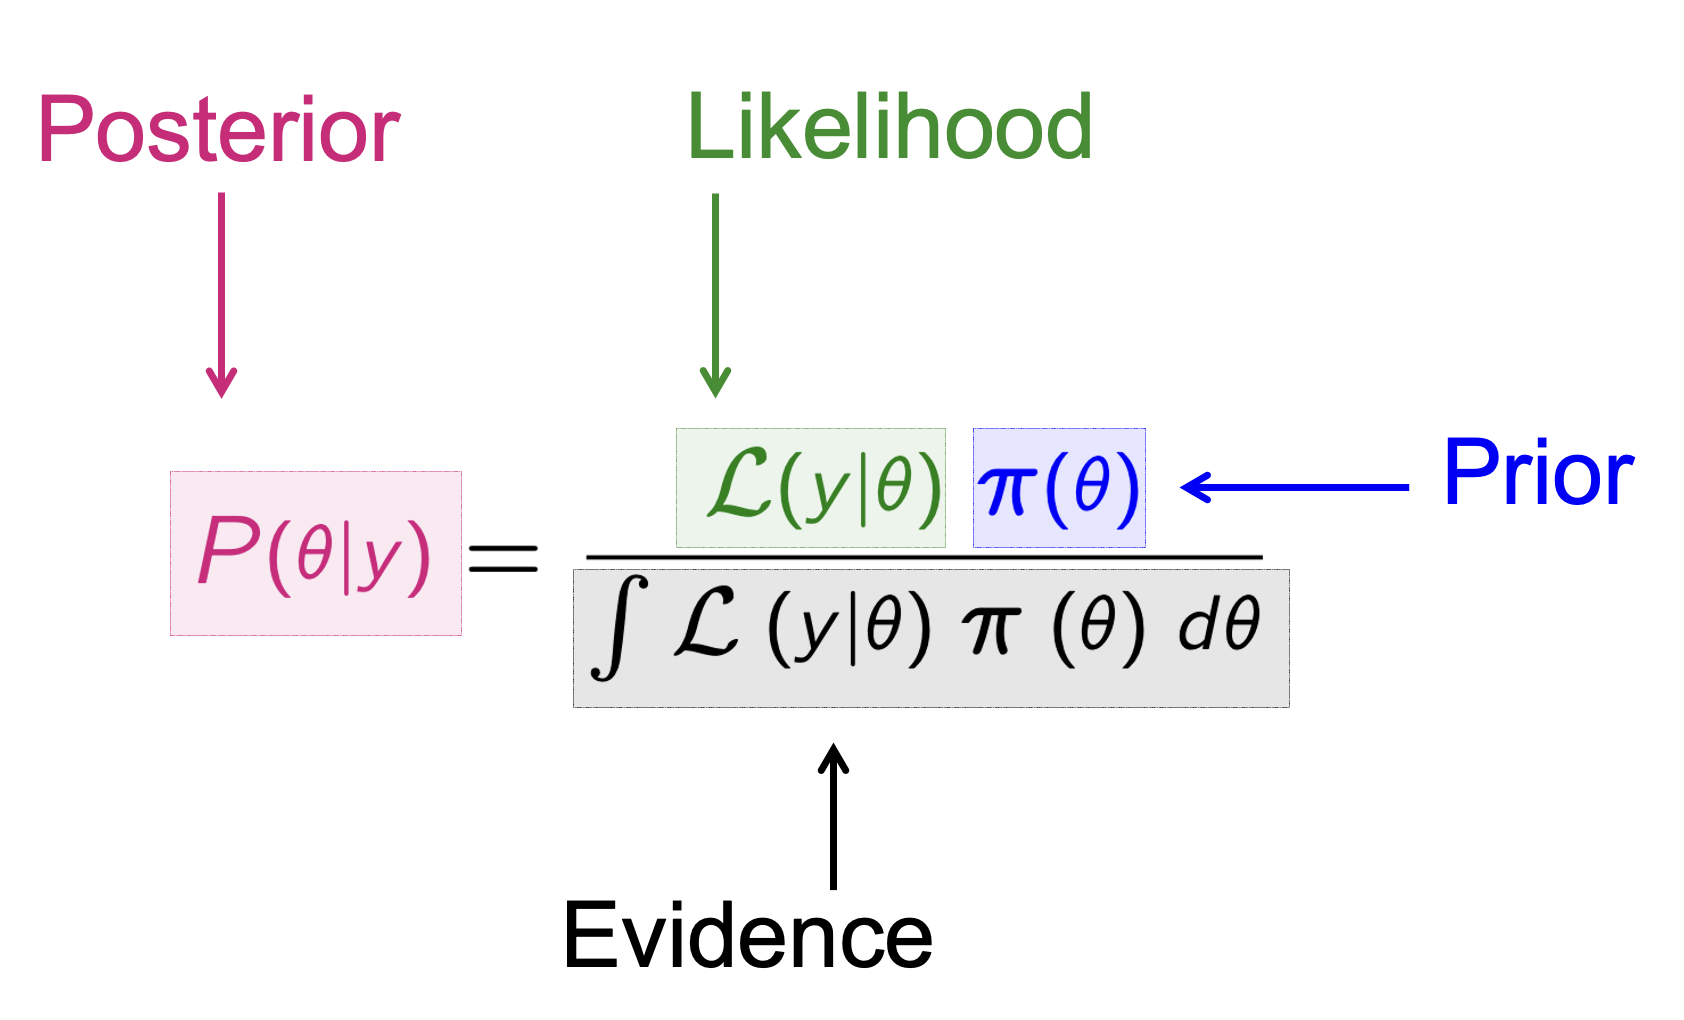
\includegraphics[scale=0.3]{BayesPic}
\end{center}
%\Large
%$ \gbl{ \mathcal{L}_{ \vwee{\theta}}  = \prod\limits_i^N f_Y (y_{_i}; \theta)  } $\\[3ex]

\end{frame} 



% PREAMBLE
\section*{Bayes Revisited}


%% BAYES
%\begin{frame}{Bayes Theorem}
%\Large
%%\begin{center}
%$\magtn{P\wee{(\theta|y)} }  =  \dfrac{ 
% \gbl{
% \mathcal{L}\wee{(y|\theta)} } \; \bbl{\pi\wee{(\theta)} }
%  } {
%  \int \mathcal{L}\wee{(y|\theta)}  \pi\wee{(\theta)}\wee{d\theta}
%  }$\\[3ex]
%
%%$\magtn{Posterior}  =  \dfrac{  \gbl{Likelihood}  \cdot \bbl{Prior}}  { Evidence }$\\[3ex]
%%%\end{center}
%\end{frame} 




%\begin{frame}{Workshop 1 Example}
%\footnotesize
%%
%%$\magtn{P\wee{(\theta|y)} }  =  \dfrac{ 
%% \gbl{
%% \mathcal{L}\wee{(y|\theta)} } \; \bbl{\pi\wee{(\theta)} }
%%  } {
%%  \int \mathcal{L}\wee{(y|\theta)}  \pi\wee{(\theta)}\wee{d\theta}
%%  }$\\[2ex]
%%  
%%$\magtn{P\wee{(\theta_+ | y_{+})} }  = 
%%\dfrac{ 
%% \gbl{  \mathcal{L}\wee{(y_{+}|\theta_{+} )}  } \; 
%% \bbl{  \pi\wee{(\theta_{+})}  } 
%%  } {
%%  \mathcal{L}\wee{(y_{+}|\theta_{+})}  \pi\wee{(\theta_{+})} + \mathcal{L}\wee{(y_{+}|\theta_{-})}  \pi\wee{(\theta_{-})}
%%  }$\\[2ex]
%%  
% $\gbl{  \mathcal{L}\wee{(y_{+}|\theta_{+})}  } =1$: `all sick people test positive'.\\[1ex]
% $\bbl{  \pi\wee{(\theta_{+})}  } =0.001$: `one in a thousand people are sick'.\\[1ex]
% $\mathcal{L}\wee{(y_{+}|\theta_{-})} = 0.05$: `one in twenty healthy people test positive'.\\[1ex]
%  $\pi\wee{(\theta_{-})}=0.999$: `999 in a thousand people are healthy'.\\[1ex]
%  
%We found the Bayesian Posterior probability (for really being $\theta_{+}$ if you test $y_{+}$) to be $\magtn{P\wee{(\theta_{+} |y_{+})} } = 0.0196 \approx 2\%$. Frequentist would say $\magtn{P\wee{(\theta_{+} |y_{+})} } = \gbl{  \mathcal{L}\wee{(y_{+}|\theta_{+})}  } = 1$.\\[1ex]
%
%\scriptsize
%\yhl{\rbl{Cowboy alert! Results are meaningless without uncertainties...}}\\
%\end{frame} 


\begin{frame}{Workshop Example}
\small
\begin{center}
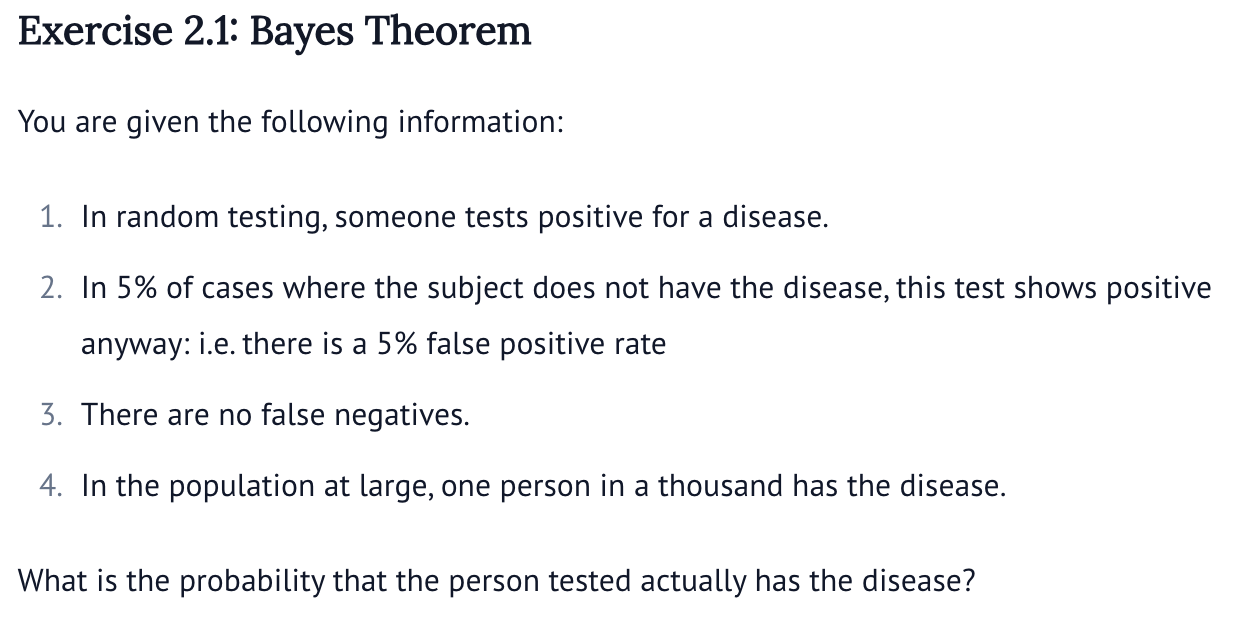
\includegraphics[scale=0.45]{w2w.png}
\end{center}
\end{frame}




%TABLES 1
\begin{frame}{Data Labels and Outcome Values}
\small
\begin{center}
\begin{tabular}{LLLL}
 %& \multicolumn{2} {C} { \overbrace{\hspace{2cm}}^{\textbf{\normalsize Data,y}} }\\
\textbf{Hypothesis} & \textbf{Negative} & \textbf{Positive}  \\[1ex]

\cellcolor{lpink} \textbf{Sick}  & \cellcolor{lpink} False\; Negative  & \cellcolor{lpink}  True\; Positive \\
  & \cellcolor{lpink} p=0  & \cellcolor{lpink}  p=1 \\
 \multicolumn{3} {C} { }\\
\cellcolor{lgreen}\textbf{Healthy}  & \cellcolor{lgreen}True\; Negative & \cellcolor{lgreen}False\; Positive \\
 & \cellcolor{lgreen}p=0.95 & \cellcolor{lgreen}p=0.05 \\
\end{tabular}


\end{center}
\end{frame}


%\begin{frame}{Outcome Values}
%\small
%\begin{center}
%\begin{tabular}{LLLL}
%\textbf{Hypothesis} & \textbf{Negative} & \textbf{Positive}  \\[1ex]
%
%\cellcolor{lpink} \textbf{Sick}  & \cellcolor{lpink} p=0  & \cellcolor{lpink}  p=1 \\
% \multicolumn{3} {C} { }\\
%\cellcolor{lgreen}\textbf{Healthy}  & \cellcolor{lgreen}p=0.95 & \cellcolor{lgreen}p=0.05 \\
%\end{tabular}
%\end{center}
%\end{frame}


\begin{frame}{Probabilities}
\small
\begin{center}
\begin{columns}

\begin{column}{0.5\textwidth}
Data are Bernoulli - binary outcome of single test.\\[1ex]


\begin{tabular}{LLLL}
\textbf{Hypothesis} & \textbf{Negative} & \textbf{Positive}  \\[1ex]

\cellcolor{lpink} \textbf{Sick}  & \cellcolor{lpink} p=0  & \cellcolor{lpink}  p=1 \\
 \multicolumn{3} {C} { }\\
\cellcolor{lgreen}\textbf{Healthy}  & \cellcolor{lgreen}p=0.95 & \cellcolor{lgreen}p=0.05 \\
\end{tabular}
\vspace{1cm}

\end{column}
\begin{column}{0.5\textwidth}
\begin{center}

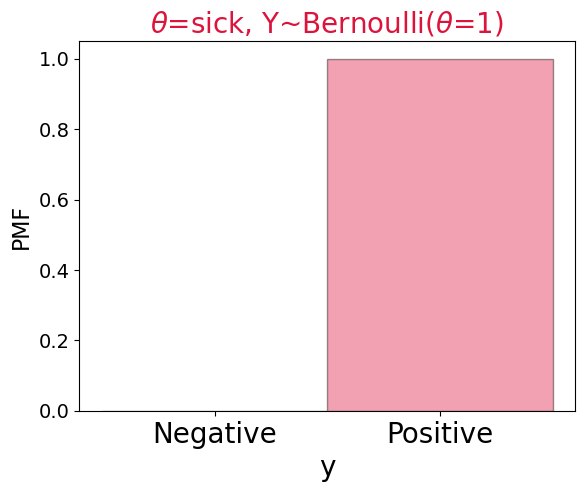
\includegraphics[scale=0.25]{NewBernCovid_sick.png}

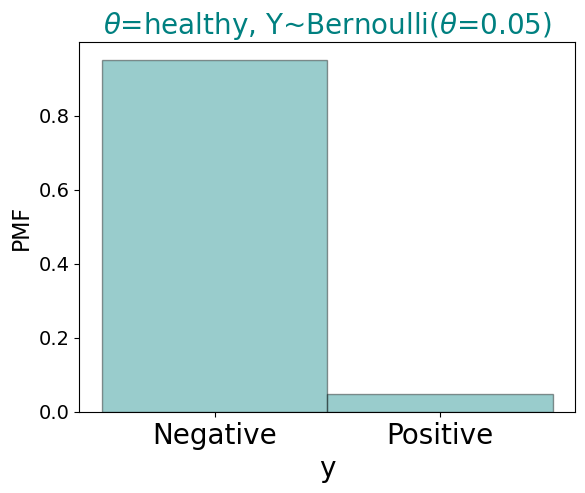
\includegraphics[scale=0.25]{NewBernCovid_healthy.png}

\end{center}
\end{column}
\end{columns}

\end{center}
\end{frame}


\begin{frame}{Recap: $Y\sim Bernoulli(\theta)$}
\footnotesize


\begin{center}
\begin{columns}

\begin{column}{0.5\textwidth}

 \yhl{$p_Y(y|\theta) =\gbl{\theta^y} \rbl{(1-\theta)^{1-y}}$}\\[1ex]
 \yhl{$\mathcal{L}( y | \theta )= p_Y(y | \theta )$ for N=1}\\[1ex]

\vspace{0.5cm}

\magtn{PMF for sick people has $\theta_+ = 1$}:\\[1ex]

$\mathcal{L}(y_+ | \theta_+) = \gbl{1^{1}} \rbl{(0)^{0} } =1 $\\[1ex]

$\mathcal{L}(y_- | \theta_+) =1 - \mathcal{L}(y_+ | \theta_+)  =  0$\\[2ex]

\vspace{0.5cm}

\tbl{PMF for healthy people has $\theta_- = 0.05$}:\\[1ex]

$\mathcal{L}(y_+ | \theta_-) = \gbl{0.05^{1}} \rbl{(0.95)^{0} } =0.05$\\[1ex]

$\mathcal{L}(y_- | \theta_-) = 1 - \mathcal{L}(y_+ | \theta_-) =  0.95$\\[1ex]

%$\mathcal{L}(y_+ | \theta_-) = \gbl{0.05^1} \rbl{0.95^0} =0.05$\\[1ex]


\vspace{1cm}

\end{column}
\begin{column}{0.5\textwidth}
\begin{center}

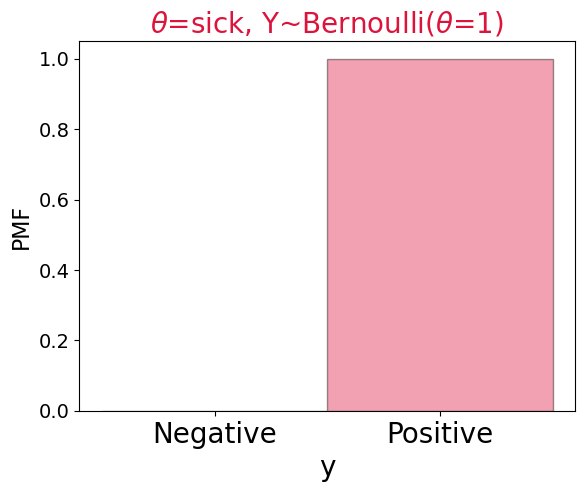
\includegraphics[scale=0.25]{NewBernCovid_sick.png}

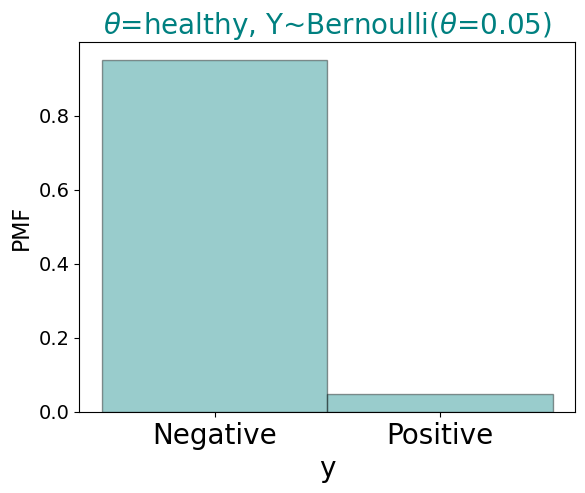
\includegraphics[scale=0.25]{NewBernCovid_healthy.png}

\end{center}
\end{column}
\end{columns}
\end{center}
\end{frame}


% LIKELIHOOD TABLE
\begin{frame}{Likelihood Table for positive tests}
\small
\begin{center}

\begin{columns}

\begin{column}{0.5\textwidth}


\begin{tabular}{LLLL}
\textbf{Hypothesis}& \textbf{Likelihood of $y_{+}$}    \\[1ex]
\cellcolor{lpink} \theta_{+} &\cellcolor{lpink} \mathcal{L}(y_{+} | \theta_{+} )=1  \\[1ex]
 \multicolumn{3} {C} { }\\
 \cellcolor{lgreen} \theta_{-} &\cellcolor{lgreen} \mathcal{L}(y_{+} | \theta_{-} )=0.05  \\[1ex]
\end{tabular}
\vspace{1cm}

\end{column}
\begin{column}{0.5\textwidth}
\begin{center}

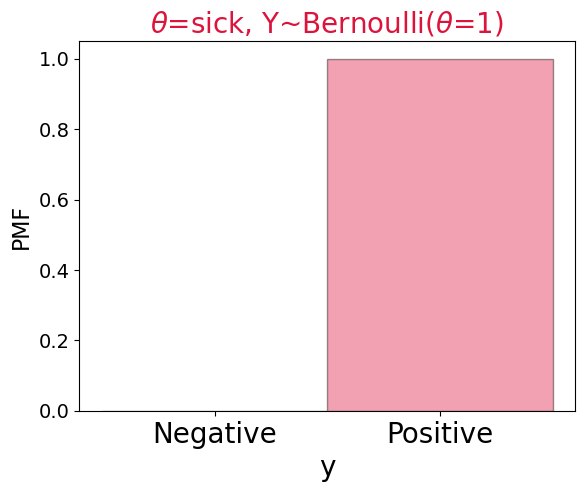
\includegraphics[scale=0.25]{NewBernCovid_sick.png}

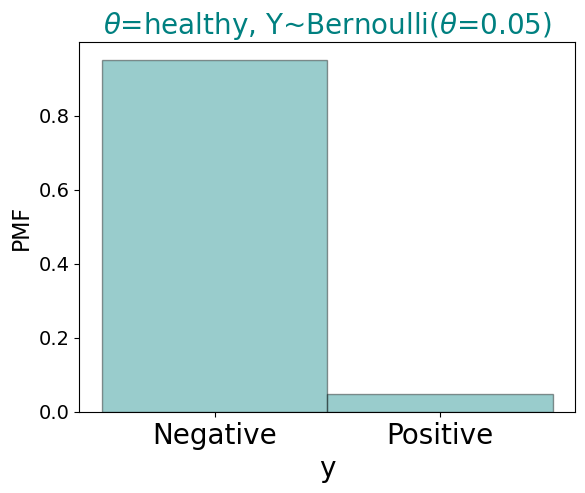
\includegraphics[scale=0.25]{NewBernCovid_healthy.png}

\end{center}
\end{column}
\end{columns}

\end{center}

\end{frame} 


% LIKELIHOOD TABLE
\begin{frame}{Likelihood Table for positive tests}
\footnotesize
\begin{center}

\begin{tabular}{LL LL LL}
\textbf{Hypothesis} & \textbf{Likelihood} & \textbf{Prior} & Bayes\; Numerator & Evidence & \textbf{Posterior}    \\[1ex]
\theta & \gbl{\mathcal{L}( y_{+} | \theta )} & \bbl{\pi(\theta)} & \gbl{\mathcal{L}( y_{+} | \theta )}\bbl{\pi(\theta)} & \int \mathcal{L} \pi d\theta &\magtn{P(\theta | y_{+} )}     \\[3ex]
% \multicolumn{6} {C} { }\\
\cellcolor{lpink} \theta_{+} &\cellcolor{lpink} 1  & \cellcolor{lpink} 1/1000 &\cellcolor{lpink}  0.001&\cellcolor{lpink}  0.05095 &\cellcolor{lpink} 0.0196  \\[1ex]
 \multicolumn{6} {C} { }\\
 \cellcolor{lgreen} \theta_{-} &\cellcolor{lgreen} 0.05 &\cellcolor{lgreen} 999/1000  & \cellcolor{lgreen} 0.04995&\cellcolor{lgreen}  0.05095& \cellcolor{lgreen} 0.9804\\[1ex]
\end{tabular}
\end{center}
\vspace{1cm}
\small
We calculated the Posteriors using Bayes' Theorem:\\[1ex]

$\magtn{P\wee{(\theta_+ | y_{+})} }  = 
  \dfrac{ 
 \gbl{  \mathcal{L}\wee{(y_{+}|\theta_{+} )}  } \; 
 \bbl{  \pi\wee{(\theta_{+})}  } 
  } {
  \int \mathcal{L}\wee{(y_{+}|\theta)}  \pi\wee{(\theta)} \wee{d\theta}
  }
  =
\dfrac{ 
 \gbl{  \mathcal{L}\wee{(y_{+}|\theta_{+} )}  } \; 
 \bbl{  \pi\wee{(\theta_{+})}  } 
  } {
  \mathcal{L}\wee{(y_{+}|\theta_{+})}  \pi\wee{(\theta_{+})} + \mathcal{L}\wee{(y_{+}|\theta_{-})}  \pi\wee{(\theta_{-})}
  }$\\[2ex]

\end{frame} 





%% FREQUENTIST INTERP
%\begin{frame}{Frequentist Interpretation}
%\small
%\begin{columns}
%
%\begin{column}{0.5\textwidth}
%
%\begin{tabular}{LLLL}
%\textbf{Hypothesis}, \theta & \textbf{Negative} & \textbf{Positive}  \\[1ex]
%
%\cellcolor{lpink} \textbf{Sick}  & \cellcolor{lpink} p=0  & \cellcolor{lpink}  p=1 \\
% \multicolumn{3} {C} { }\\
%\cellcolor{lgreen}\textbf{Healthy}  & \cellcolor{lgreen}p=0.95 & \cellcolor{lgreen}p=0.05 \\
%\end{tabular}
%
%The probability of you being sick if you test positive is $ P(sick | +) = \mathcal{L}(+ | sick) =1$\\[1ex]
%
%\end{column}
%\begin{column}{0.5\textwidth}
%\begin{center}
%
%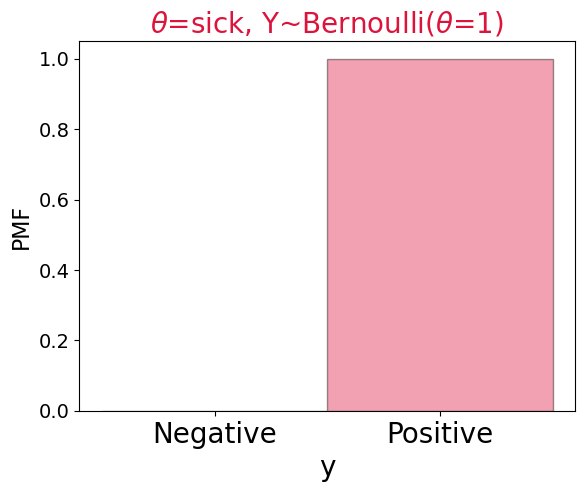
\includegraphics[scale=0.25]{NewBernCovid_sick.png}
%
%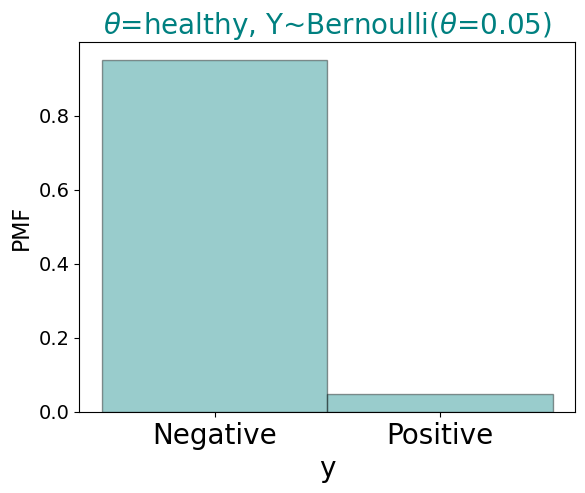
\includegraphics[scale=0.25]{NewBernCovid_healthy.png}
%
%\end{center}
%\end{column}
%\end{columns}


%\end{frame} 







%\begin{frame}{Form of Likelihood}
%\footnotesize
%In this example we had a sample of $N=1$, and our two Likelihoods $\gbl{  \mathcal{L}\wee{(k|\theta)}  }$ for our two hypotheses  were \magtn{Bernoulli}: $p_K(k) =\theta^k (1-\theta)^{1-k}$. \\[1ex]
%
%\begin{multicols}{2}
%$  \mathcal{L}\wee{(k|\rbl{sick})}   = p_K\wee{(-)} = 1-\theta = 0$\\
%
%\hspace{1.25cm} $ p_K\wee{(+)} = \theta = 1$\\[1ex]
%
%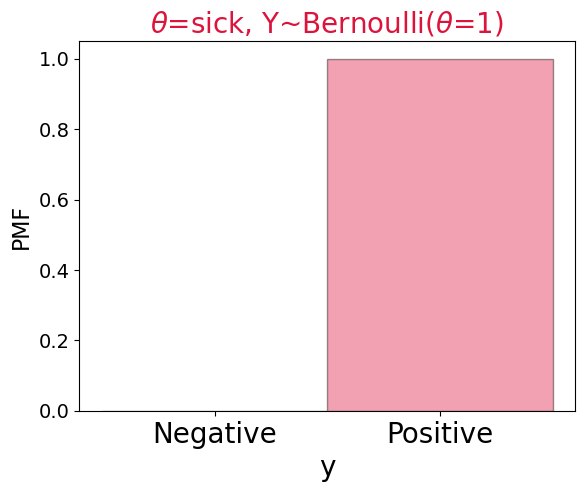
\includegraphics[scale=0.25]{NewBernCovid_sick.png}
%
%
%$\mathcal{L}\wee{(k|\gbl{healthy})}   = p_K\wee{(-)} =1-\theta = 0.95$\\
%
%\hspace{1.55cm} $ p_K\wee{(+)} = \theta = 0.05$\\[1ex]
%
%%\begin{center}
%
%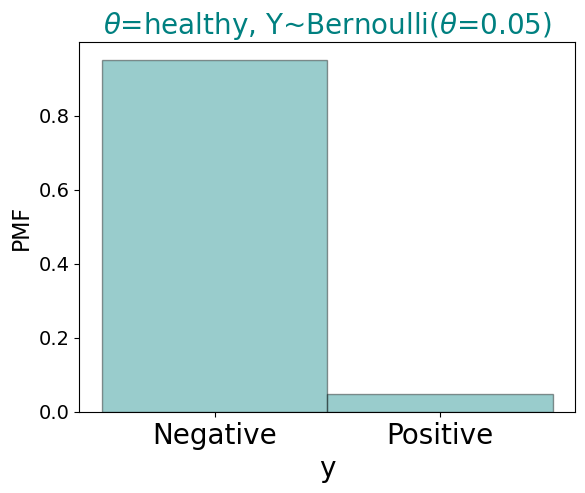
\includegraphics[scale=0.25]{NewBernCovid_healthy.png}
%%\end{center}
%\end{multicols}
%\end{frame} 


\begin{frame}{Bayesian Updating}
\small
What we did in the workshop is called Bayesian Updating.\\[1ex]

We updated our estimate of the probability from the $\bbl{Prior,\; \pi\wee{(\theta)}  }$, to the $\magtn{Posterior,\;P\wee{(\theta|y)}}$.\\[1ex]

We did this using the data $y$, and the Likelihoods $\mathcal{L}\wee{(y|\theta)}$ provided to us by the test manufacturer for the two possible hypotheses $\theta$.\\

\begin{itemize}
\item \bbl{Before} looking at the data, we had a \bbl{Prior} $\bbl{  \pi\wee{(\theta_+)}  } =0.001$.
\item \magtn{After} the test we calculated a \magtn{Posterior} $\magtn{P\wee{(\theta_+ |y_+)}} =0.0196 \approx 0.02$.
\end{itemize}

\vspace{0.5cm}
\yhl{\rbl{Cowboy alert! Results are meaningless without uncertainties...}}\\

\end{frame} 


\begin{frame}{Evidence}
\small
Recall that we need the Evidence (Bayes denominator) to ensure the Posterior is a valid PDF: $\int \magtn{P\wee{(\theta|y)}}\, d\theta =1$. \\[1ex]

$\magtn{P\wee{(\theta_+ | y_{+})} }  = 
  \dfrac{ 
 \gbl{  \mathcal{L}\wee{(y_{+}|\theta_{+} )}  } \; 
 \bbl{  \pi\wee{(\theta_{+})}  } 
  } {
  \int \mathcal{L}\wee{(y_{+}|\theta)}  \pi\wee{(\theta)} \wee{d\theta}
  }
  = \gbl{  \mathcal{L}\wee{(y_{+}|\theta_{+} )}  } \; 
 \bbl{  \pi\wee{(\theta_{+})}  } \times \grhl{c} 
$\\[2ex]
  
  

However, it is just a \grhl{constant factor}, identical for every hypothesis,  so we could \rbl{make life easier for ourselves}:\\

\begin{itemize}
\item $\magtn{P\wee{(\theta_+ | y_{+})}  }  =  \gbl{ \mathcal{L}\wee{(y_{+}|\theta_{+} )}   }\;\bbl{  \pi\wee{(\theta_{+})}   } \,  \grhl{c}
= \gbl{ 1} \times \bbl{ 0.001}\,\grhl{c}
= 0.001\grhl{c}$

\item $\magtn{P\wee{(\theta_- | y_{+})}  }  =  \gbl{ \mathcal{L}\wee{(y_{-}|\theta_{+} )}   }\;\bbl{  \pi\wee{(\theta_{+})}  } \,  \grhl{c}
= \gbl{ 0.05} \times \bbl{ 0.999}\,\grhl{c}
= 0.04995\grhl{c}$

%\item $\magtn{P\wee{(healthy|+)} }  =  \gbl{  \mathcal{L}\wee{(+|healthy)}  } \;\bbl{   \pi\wee{(\theta_{-})}   } \times  \grhl{c}
%= \gbl{ 0.05} \times \bbl{ 0.999}\times \grhl{c}
%= 0.04995\grhl{c}$
\item $\int \magtn{P\wee{(\theta|y_+)}}\, d\theta =  0.05095\,\grhl{c} = 1\;\; \therefore$ \grhl{$c\approx19.627$}
\end{itemize}
\vspace{0.5cm}

This shortcut gives us \magtn{Posteriors} of (0.0196, 0.9804) as before.\\[1ex]

\end{frame} 

\begin{frame}
\small
\begin{center}
\only<1>{ 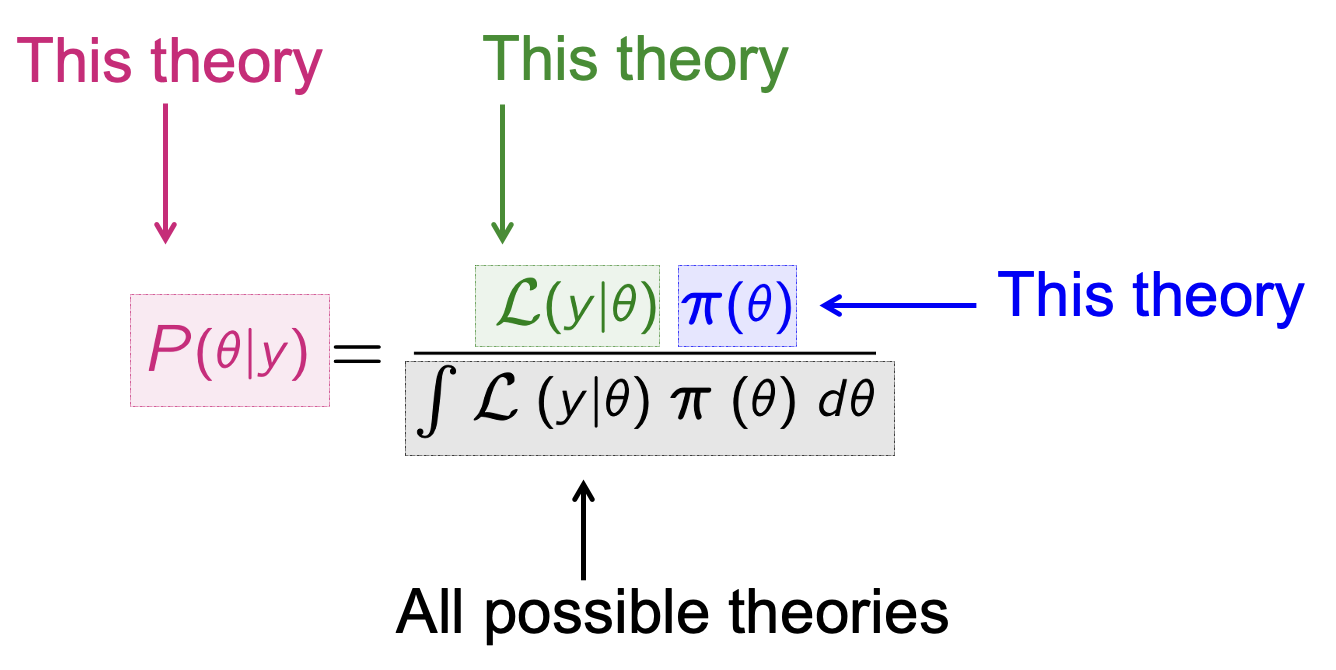
\includegraphics[scale=0.45]{BL1.png} }
\only<2>{ 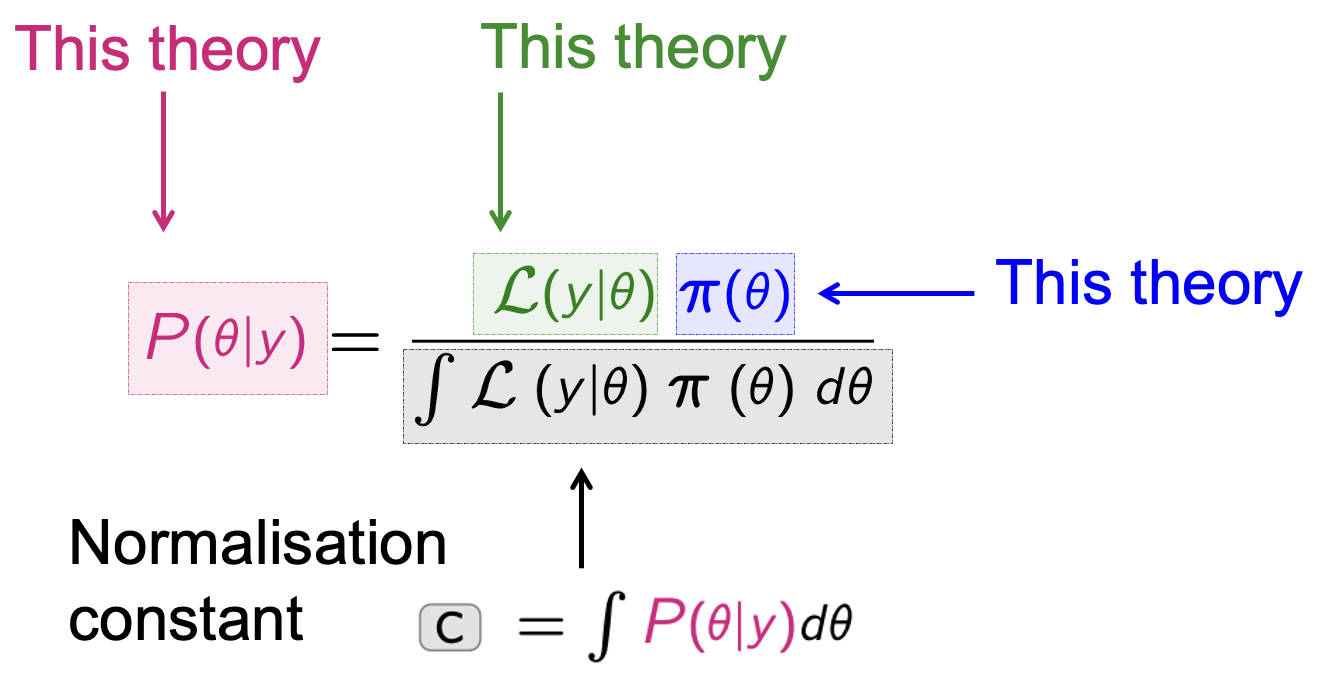
\includegraphics[scale=0.45]{BL2.png} }
\only<3>{ 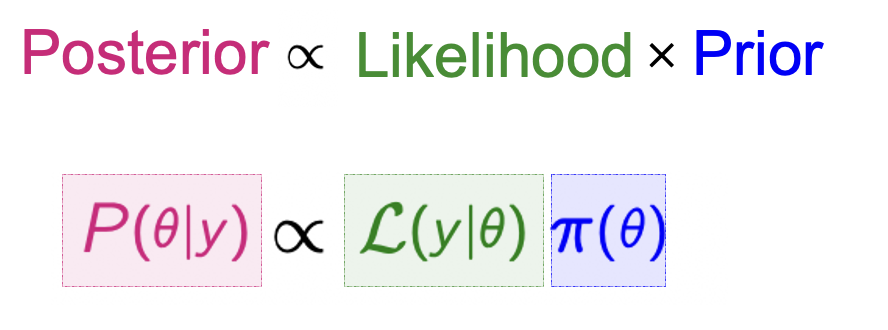
\includegraphics[scale=0.45]{BL3.png} }
\end{center}
\end{frame} 

\section*{Prior PDF, MAP, CI}

\begin{frame}{Form of Prior}
\small
For our Priors, we assigned $\pi\wee{(\theta_-)}=999/1000$ and $\pi\wee{(\theta_+)}=1/1000$.\\[1ex]

\rbl{This was a very specific choice, made as though we could know with absolute certainty the rate of cases at that given time, which is of course impossible.}\\[1ex]

The Prior probability should be a PDF\magtn{*} with some specific distribution in the range [0,1]. This is what the \magtn{Beta($\alpha, \beta$)} distribution is made for.\\[1ex]

%For this example we could estimate $\pi\wee{(\theta_+)}= (\bbl{1} \pm \gbl{0.5})/1000$.\\[1ex]
%
% This means we want our prior distribution to have $E[\theta]=\bbl{1\times10^{-3}}$ and $V[\theta] = (\gbl{0.5\times10^{-3}})^2 = 2.5\times10^{-7}$.\\[1ex]
%
%\scriptsize
\magtn{* If the prior is not a valid PDF, it is an `Improper Prior' - these can still be used.}
\end{frame} 



\begin{frame}{Recap: $Y\sim Beta(\alpha,\beta)$\hfill \footnotesize  \bhl{$f_{\theta}(\theta) = \frac{1}{B(\alpha,\beta)}\, \theta^{\alpha-1} (1-\theta)^{\beta-1}$}}
\footnotesize
Recall the Beta($\alpha, \beta$) distribution is a chameleon, being able to take on a huge range of shapes depending on its two shape hyper-parameters $\alpha, \beta$.\\

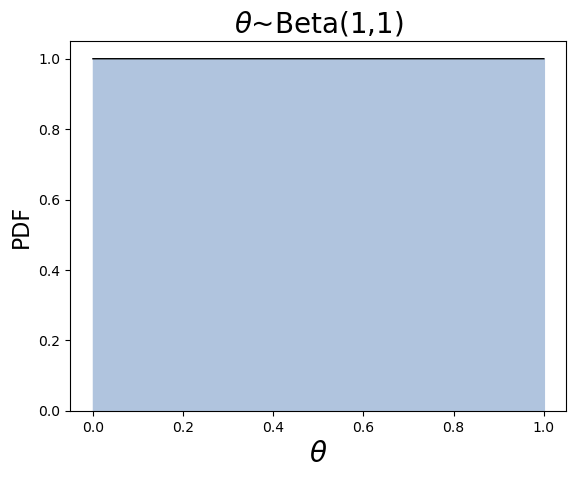
\includegraphics[scale=0.23]{Beta1_1.png}
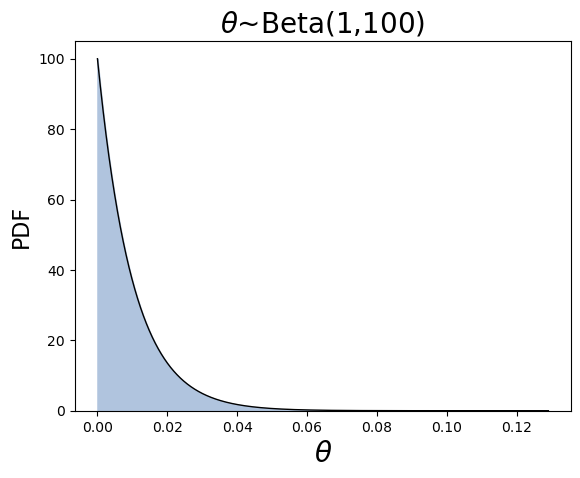
\includegraphics[scale=0.23]{Beta1_100.png}
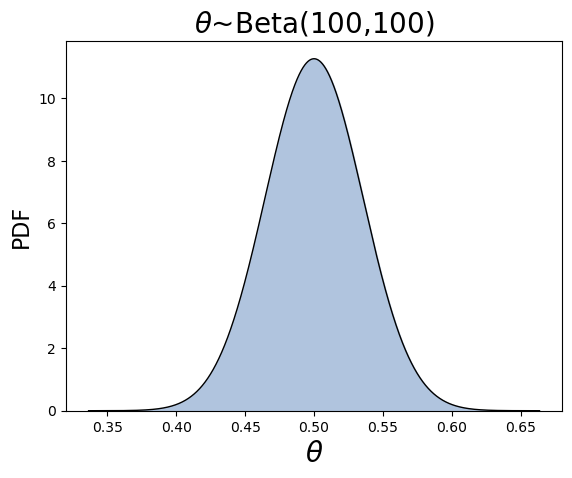
\includegraphics[scale=0.23]{Beta100_100.png}

The $B(\alpha,\beta)$ in the PDF ensures normalisation.\\[1ex]
\grhl{\texttt{ from scipy.special import beta as betafunc}} (same name as the scipy.stats beta distribution - careful!):\\[1ex]
\grhl{\texttt{betafunc(1,1)=1}}; \grhl{\texttt{betafunc(0.1, 99.9)=6.006}} etcetera.\\[1ex]
\end{frame} 




\begin{frame}{Recap: $Y\sim Beta(\alpha,\beta)$\hfill \footnotesize  \bhl{$f_{\theta}(\theta) = \frac{1}{B(\alpha,\beta)}\, \theta^{\alpha-1} (1-\theta)^{\beta-1}$}}
\footnotesize
Recall the Beta($\alpha, \beta$) distribution is a chameleon, being able to take on a huge range of shapes depending on its two shape hyper-parameters $\alpha, \beta$.\\

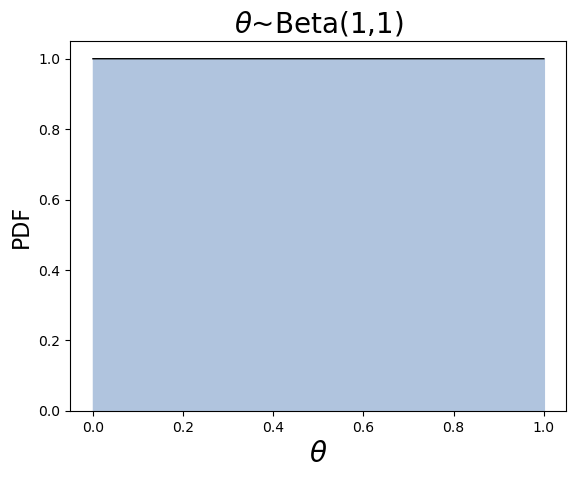
\includegraphics[scale=0.23]{Beta1_1.png}
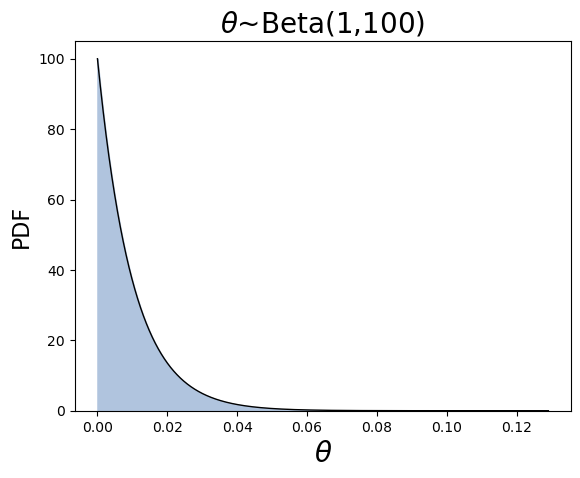
\includegraphics[scale=0.23]{Beta1_100.png}
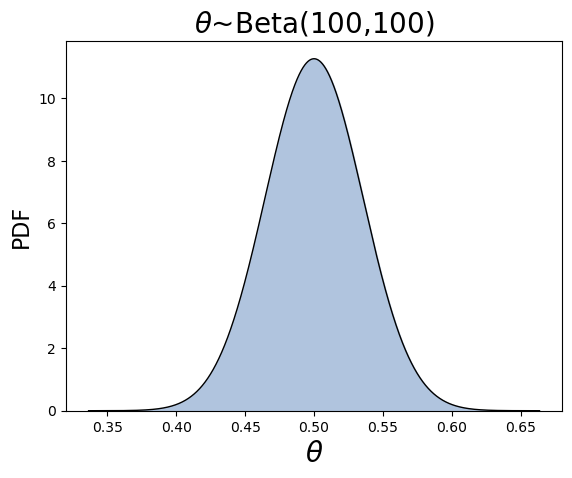
\includegraphics[scale=0.23]{Beta100_100.png}

\rbl{PDF}: $f_{\theta}(\theta) \propto \theta^{\alpha-1} (1-\theta)^{\beta-1}$ \bbl{with $0\leq \theta \leq 1$, $\alpha>0$, $\beta>0$}\\[1ex]

\rbl{Expected Value}: \ghl{$E[\theta] = \dfrac{\alpha}{\alpha+\beta}$} and \rbl{Variance}: \ghl{$V[\theta] = \dfrac{E[\theta](1-E[\theta])}{(\alpha +\beta+1)}$}\\[1ex]

\end{frame} 





%\begin{frame}{Beta Prior for covid prevalence}
%\small
%\yhl{$E[\theta] = \dfrac{\alpha}{\alpha+\beta}$} and \yhl{$V[\theta] = \dfrac{E[\theta](1-E[\theta])}{(\alpha +\beta+1)}$}\\[1ex]
%
%To use Beta as our prior we want $E[\theta]=1\times10^{-3}$ and $V[\theta] \approx 2.5\times10^{-7}$.\\[1ex]
%
%For $E[\theta] = \dfrac{\alpha}{\alpha+\beta} = 1\times10^{-3}$\;\; \rbl{\ding{234}\; try $\alpha=0.1$, $\beta = 99.9$}\\[1ex]
%
%For these values of $\alpha, \beta$ we find $V[\theta] = 9.89\times10^{-6}$ - that'll do.\\[1ex]
%
%We will try with:\\[1ex]
%\bbl{$\pi\wee{(\theta_+)} = Beta(0.1,99.9)$}\;\; and\;\; \bbl{$\pi\wee{(\theta_-)} = Beta(99.9,0.1)$}.\\[1ex]
%
%\rbl{*First I tried the more obvious (1,999) and got a tiny variance, and tiny posterior.}
%%Note the expected values are $E[\pi\wee{(sick)}]
%
%\end{frame} 






% THE POSTERIOR
\begin{frame}{The Posterior  \;\;$
\magtn{ P\wee{(\theta | y )} } \propto  
\gbl{ \mathcal{L}\wee{ (y|\theta) } } 
\;\bbl{ \pi\wee{(\theta)}}
$ }
\small
Beta Priors: \bbl{$\pi\wee{(\theta)}= \propto\, \theta^{\alpha-1} (1-\theta)^{\beta-1}$}\\[1ex]
Bernoulli Likelihoods: \gbl{$\mathcal{L}\wee{(y|\theta)} = \theta^{y} (1-\theta)^{1-y} $} (for N=1 data point)\\[1ex]
\footnotesize
\begin{align*}
\mathsf{The\; Posterior:\;} \magtn{ P\wee{(\theta | y )} } 
& \propto  
\gbl{ \mathcal{L}\wee{ (y|\theta) } } 
\;\bbl{ \pi\wee{(\theta)}} \hspace{4cm}\\[0.5ex]  
& \propto \,
\gbl{ \theta^{y} (1-\theta)^{1-y} }
\;\bbl{ \theta^{\alpha-1} (1-\theta)^{\beta-1} } \\[0.5ex]  
& \propto \,
\gbl{\theta^{y}}\bbl{\theta^{\alpha -1}} \;\gbl{(1-\theta)^{1-y}}\bbl{(1-\theta)^{\beta - 1}}  \hspace{5cm}\\
& \propto \,
\theta^{y +\alpha -1} \;(1-\theta)^{1-y + \beta - 1}  \hspace{5cm}\\
& \propto \,
\theta^{(\alpha+[y])-1} \;(1-\theta)^{(\beta+[1-y])-1}  \hspace{5cm}\\
& \propto \,
\magtn{ \theta^{\alpha'-1} \;(1-\theta)^{\beta'-1} } \hspace{5cm}\\
\end{align*}
\small

The Posterior \magtn{$P\wee{(\theta | y )}\propto Beta(\alpha', \beta')$} where $\alpha'=\alpha+[y]$ and $\beta' = \beta+[1-y]$.\\[1ex]
Bernoulli and Beta are Conjugate: \bhl{\magtn{Beta} =\gbl{Bernoulli} $\times$ \bbl{Beta} }.\\[1ex]

\end{frame}


% BETA BERNOULLI
\begin{frame}{The Posterior}
\small
Priors: \bbl{$\pi\wee{(\theta)}  \propto\, \theta^{\alpha-1} (1-\theta)^{\beta-1}$}\\[1ex]

Posteriors: \magtn{$P\wee{(\theta | y )} \propto \theta^{(\alpha+[y])-1} \;(1-\theta)^{(\beta+[1-y])-1}$}\\[1ex]

If $y=0$:\;\; \magtn{$P\wee{(\theta | y=0 )}\propto \theta^{\alpha-1} \;(1-\theta)^{[\beta+1] -1}$}\\[1ex]
\ding{234}\;\; A negative result increments $\beta \rightarrow [\beta+1]$ wrt prior.\\[1ex]

If $y=1$:\;\; \magtn{$P\wee{(\theta | y=1 )}\propto \theta^{[\alpha+1]-1} \;(1-\theta)^{\beta-1}$}\\[1ex]
\ding{234}\;\; A positive result increments $\alpha \rightarrow [\alpha+1]$ wrt prior.\\[1ex]

\end{frame}

%NORMALISATION CONSTANT FOR BETA
%\begin{frame}{Aside: The Normalisation Constant}
%\small
%\yhl{$ f(\theta | \alpha,\beta) = \dfrac{1}{B(\alpha,\beta)} \theta^{\alpha-1} (1-\theta)^{\beta-1}$}\\[1ex]
%
%The normalisation is the Beta function: 
%
%$B(\alpha,\beta) = \int\limits_0^1 \theta^{\alpha-1} (1-\theta)^{\beta-1} d\theta 
%= \dfrac{\Gamma(\beta)\Gamma(\alpha)}{ \Gamma(\alpha+\beta)}$\\[1ex]
%
%%The nice properties of this function include \magtn{$\Gamma(1/2)  = \sqrt{\pi}$},  \bbl{$\Gamma(n ) = (n-1)!$ where $n$ is a positive integer}, and \gbl{$\Gamma(s+1)  = s\Gamma(s)$}.\\[1ex]
%
%%For our Posterior and $y=1$ (test is positive) we have $\alpha'=\alpha+y = 1.1$ and $\beta' = \beta-y+1 = 99.9$.\\[1ex]
%We can calculate the Normalisation on our prior with the beta function provided by \texttt{from scipy.special import beta as betafunc} (same name as the scipy.stats beta distribution - careful!):\\[1ex]
%
%For the prior: \grhl{\texttt{betafunc(0.1, 99.9) = 6.006}}\\[1ex]
%For the posterior: \grhl{\texttt{betafunc(1.1, 99.9) = 0.006}}\\[1ex]
%
%
%We find \grhl{$c_{\pi} = 6.006/0.006 \approx 0.001$}\\[1ex]
%
%
%\end{frame}


 
 

% POSTERIOR FOR COVID TEST
\begin{frame}{The Posterior Expectation for the Covid Test}
\small
We cannot use the formula for the Posterior directly with $\theta=1$ and $y=1$, as it would give us a zero posterior for any value of $\beta \neq 1$.\\[1ex]
%
$P(\theta | y ) \propto \theta^{(\alpha+y)-1} \;(1-\theta)^{(\beta-y+1)-1}$\\

$P(\theta=1 | y=1 ) \propto  1^{\alpha} \;(0)^{\beta-1} $\;\;\yhl{\rbl{\ding{234} only non-zero for $\beta=1$.}}\\[1ex]

\magtn{Could we use a $Beta(\alpha, 1)$?} %We want a Beta distribution that has an expectation value = 0.001, our prior knowledge or the prevalence of covid in the community.\\[1ex]

We want $E[\theta] = \dfrac{\alpha}{\alpha+\beta} = \dfrac{\alpha}{\alpha+1} = 0.001$\\[1ex]

A value $\alpha = 0.\overline{001}$ satisfies this. Let's have a look at the distribution.

%Let's look at the variance:\\[1ex]

%$V[\theta] = \dfrac{ E[\theta] (1-E[\theta] ) }{\alpha+\beta+1}  = 0.0005$\\[1ex]



\end{frame}

% POSTERIOR FOR COVID TEST
\begin{frame}{The Posterior Expectation for the Covid Test}
\footnotesize

\begin{columns}
\begin{column}{0.5\textwidth}
The $Beta( 0.\overline{001}, 1)$ is almost entirely concentrated at values below $10^{-7}$. \\[2ex]
\vspace{0.2cm}

The tail extends to 1, enabling the expectation $E[\theta]=10^{-3}$.\\[2ex]
\vspace{0.1cm}

The Posterior expectation is 
$E[P] = \dfrac{\alpha+1}{\alpha+1+\beta} =  \dfrac{1.\overline{001}}{2.\overline{001}}\approx 0.5$\\[2ex]


\end{column}
\begin{column}{0.6\textwidth}

\begin{center}
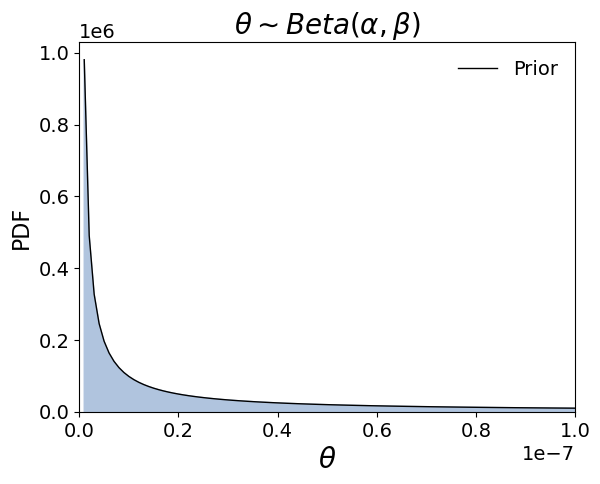
\includegraphics[scale=0.4]{CovidBetaBernoulli0.001001001001_1.png}
\end{center}

\end{column}
\end{columns}

\magtn{This is not a distribution I would choose to model prevalence of a disease!} 
\end{frame}





% POSTERIOR FOR COVID TEST
%\begin{frame}{The Posterior Expectation for the Covid Test}
%\small
%We cannot use the formula for the Posterior directly with $\theta=1$ and $y=1$, as it would give us a zero posterior for any value of $\beta \neq 1$\magtn{*}.\\[1ex]
%%
%$P(\theta | y ) = c_{\pi}\, \theta^{(\alpha+y)-1} \;(1-\theta)^{(\beta-y+1)-1}$\\
%
%$P(\theta_{+} | y_{+} ) = c_{\pi}\, 1^{1.1} \;(0)^{99.9} = 0$\yhl{\rbl{\ding{234} our toy will not work here.}}\\[1ex]
%
%
%We can look at the posterior expected value, though, using the expectation for a Beta:\\[1ex]
%
%\bhl{$E[X] = \dfrac{\alpha}{\alpha+\beta}$ for $X \sim Beta(\alpha, \beta)$}\\[1ex]
%
%
%\scriptsize
%\magtn{*This helps us understand the unique form of the Bernoulli PMF: $\theta^{y} (1-\theta)^{1-y}$, which ensures the second term is $0^0=1$ when $y=1$}.\\[1ex]
%
%
%\end{frame}
%
%
%
%
%
%
%% POSTERIOR FOR COVID TEST
%\begin{frame}{The Toy Posterior for the Covid Test}
%\small
%For a positive test $y=y_+=1$, and for being sick $\theta=\theta_+$ we have posterior hyper-parameters $\alpha=1.1, \beta=99.9$\\[1ex]
%
%$E [ \magtn{ P\wee{ (\theta_+ | y_+ ) } } ] \approx 1\% $\;\; (\rbl{compare: $2\%$}).\\[1ex]
%
%Why is it lower? \\[1ex]
%
%In the workshop we used the prior 0.001 to weight our single measurement. We took into account the false positive rate for the Evidence in the denominator, and found a scale factor of c=19.627.This scale factor multiplied by the prior gave us a posterior of 0.02.\\[1ex]
%
%
%
%
%\end{frame}



% POSTERIOR FOR COVID TEST
%\begin{frame}{The Toy Posterior for the Covid Test}
%\small
%For a positive test $y=y_+=1$, and for being sick $\theta=\theta_+$ we have posterior hyper-parameters $\alpha=1.1, \beta=99.9$\\[1ex]
%
%$E [ \magtn{ P\wee{ (\theta_+ | y_+ ) } } ] \approx 1\% $\;\; (\rbl{compare: $2\%$}).\\[1ex]
%
%
%Why is it lower? 
%
%I made it lower with my daft model, which uses a prior that looks like this:
%
%\begin{center}
%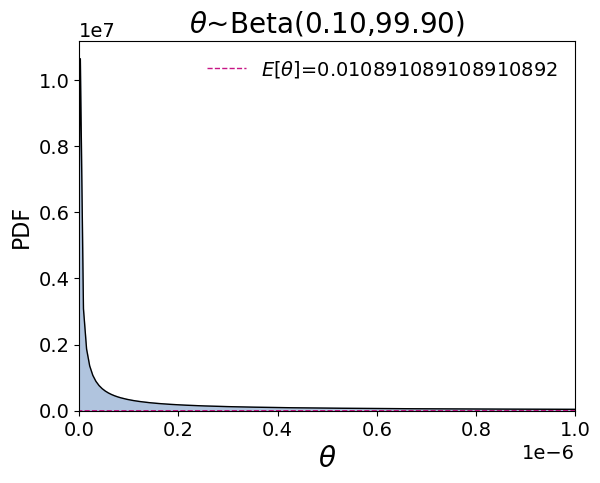
\includegraphics[scale=0.3]{CovidBetaBernoulli0.1_99.9.png}
%\end{center}
%
%\yhl{\rbl{Always look at the prior distribution! You can get a sensible expectation and variance from a total dog.}}
%
%\end{frame}




%%UNIFORM PRIOR
%\begin{frame}{Insights}
%\small
%The Beta-Bernoulli Posterior \magtn{$P\wee{(\theta | y )}\propto Beta(\alpha', \beta')$} where $\alpha'=\alpha+y$ and $\beta' = \beta-y+1$.\\[1ex]
%
%What if we had used a Uniform Prior, $Beta(1,1)$?\\[1ex]
%
%With this simple case, it is easier to see the relationship between the Posterior, Prior, and Data.\\[1ex]
%
%If my single measurement is a positive $y=1$, I add 1 to $\alpha$. The posterior is $Beta(\alpha+1, \beta) = Beta(2,1)$.\\[1ex]
%
%The Expected Value is then $E[\theta] = \dfrac{2}{3}$: this has moved upwards from its original $E[\theta] = \dfrac{1}{2}$ because of the data.\\[1ex]
%
%If my single measurement is a negative $y=0$, I add 1 to $\beta$. The posterior is $Beta(\alpha, \beta+1) = Beta(1,2)$.\\[1ex]
%
%The Expected Value is then $E[\theta] = \dfrac{1}{3}$: this has moved downwards from its original $E[\theta] = \dfrac{1}{2}$ because of the data.\\[1ex]
%
% \end{frame}
 
 
 
 

\begin{frame}{All Models Are Wrong (not just these. All.)}
\small
The \magtn{Frequentist} model is that the posterior is the likelihood. \yhl{$P(\theta_+| y_+) =\mathcal{L}(y_+|\theta_+) =100\%$}.\\[2ex]

With a \magtn{Single-valued Prior} of 1/1000, the posterior is \yhl{$P(\theta_+| y_+) = 0.0196 \approx 2\%$}.\\[1ex]
This prior model suggests infinite precision and zero uncertainty, so is worrisome.\\[2ex]

With a (lazy, crazy) \magtn{Beta Prior} the posterior is \yhl{$P(\theta_+| y_+)  \approx 50\%$}.\\[1ex]
This prior model gave us $E[\theta_+]=0.001$ and a nonzero uncertainty, but clearly wasn't "the one".\\[2ex]
\bbl{ Which model is the 'wrongest'?}\\[1ex]

\end{frame}


\begin{frame}{Other choices we could have made}
\footnotesize

Insisting on an uncertainty means we must have a distribution, not a number, for our prior. Where did we get the 1/1000 prior? What are our sources of uncertainty?\\[1ex]
%
%Examples I found on the internet include:\\[1ex]
%\href{https://pmc.ncbi.nlm.nih.gov/articles/PMC10594563/}{ Wastewater sampling with kNN}

The ONS have a very good description of their 
\href{https://www.ons.gov.uk/peoplepopulationandcommunity/healthandsocialcare/conditionsanddiseases/methodologies/covid19infectionsurveypilotmethodsandfurtherinformation}{methodology}
 and a \href{https://github.com/ONSdigital/CIS_MRP_PUBLIC}{github repo} with all the data and the analysis code. This is absolutely what everyone must always do if they want their analysis to be taken seriously.\\[1ex]

It seems they used a Bayesian Posterior, and the prevalences quoted to the public were \magtn{Maximum A Posteriori} (MAP) estimates. I \href{https://www.ons.gov.uk/peoplepopulationandcommunity/healthandsocialcare/conditionsanddiseases/articles/coronaviruscovid19latestinsights/infections}{downloaded the data} and saw that around April 2021, the MAP prevalence in England was $0.1\%$ with a $95\%$ \magtn{Credible Interval} of $(0.08,0.12)\%$)\\

Based on this ten mins of research, I have adjusted my guess for the Prior: I would try a Normal (non-conjugate) Prior with mean $0.1\%$ (as before) and sigma $0.02\%$. A non-conjugate prior means we would have to solve numerically.
\end{frame}


% MAP ESTIMATION
\begin{frame}{Maximum A Posteriori Estimation}
\small
The value of $\theta$ that maximises the Posterior distribution (the mode of the posterior) is the MAP estimate. \\[1ex]

\begin{columns}
\begin{column}{0.6\textwidth}

\begin{center}
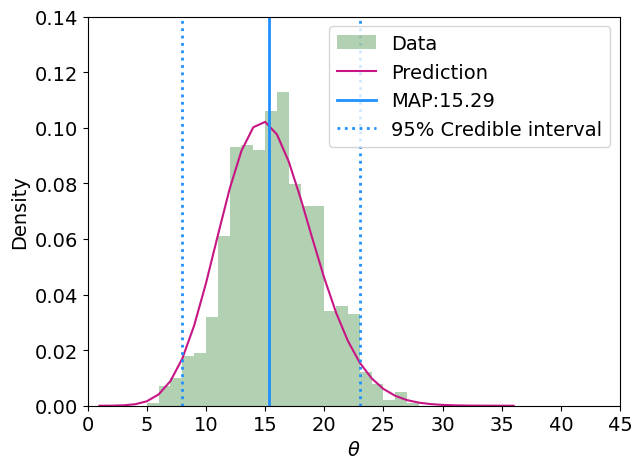
\includegraphics[scale=0.4]{mapPG-a15-b1.png}
\end{center}

\end{column}
\begin{column}{0.4\textwidth}
\footnotesize
Gamma $mode=\dfrac{\alpha'-1}{\beta'}$.\\[1ex]

Beta $mode=\dfrac{\alpha'-1}{\alpha'+\beta'+2}$.\\[1ex]

$\alpha' , \beta'$ are hyper-parameters of the Posterior distribution.
\end{column}
\end{columns}
\end{frame} 

% MAP ESTIMATION
\begin{frame}{Maximum A Posteriori Estimation}
\small
%The value of $\theta$ that maximises the Posterior distribution (the mode of the posterior) is the MAP estimate, $\thetahat_{MAP}$. \\[1ex]

 $\magtn{ P\wee{(\theta | y )} } \propto  \gbl{ \mathcal{L}\wee{ (y|\theta) } } \;\bbl{ \pi\wee{(\theta)}}$\\[1ex]
 
$\arg\max\limits_{\theta} \magtn{ P\wee{(\theta | y )} }  = \arg\max\limits_{\theta}  \gbl{ \mathcal{L}\wee{ (y|\theta) } } \;\bbl{ \pi\wee{(\theta)}}$\\[1ex]

If the Prior $\bbl{ \pi\wee{(\theta)}}$ is uniform, the $\thetahat_{MAP}$ is equivalent to the $\thetahat_{MLE}$.\\[1ex]

The difference between $\thetahat_{MAP}$ and $\thetahat_{MLE}$ is that the former uses not just data, but also our prior beliefs on the parameter's value.\\[1ex]

In the limit of large datasets, $\thetahat_{MAP} \rightarrow \thetahat_{MLE}$. The main feature (until we look at MCMC magic) of Bayesian Posterior updating is its formidable performance with tiny amounts of data.\\

\end{frame} 




% CREDIBLE INTERVALS
\begin{frame}{Credible Intervals}
\footnotesize
A \bbl{Credible Interval} is a range of values of the posterior that contain the true parameter with a certain probability, for example $95\%$. This intuitive definition is what many people incorrectly think the (unintuitive) Confidence Interval\rbl{*} is.

\begin{center}
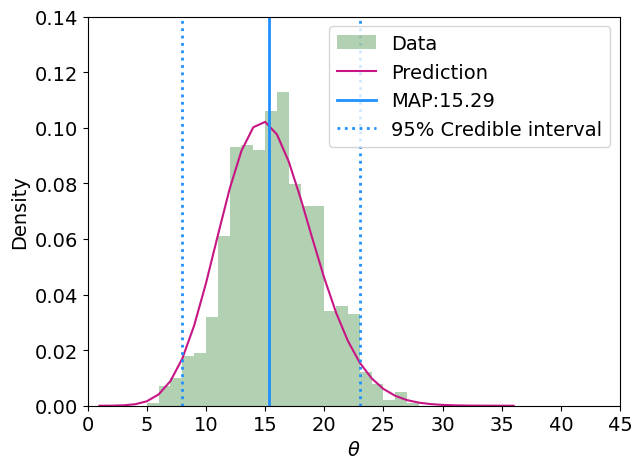
\includegraphics[scale=0.35]{mapPG-a15-b1.png}
\end{center}

\scriptsize
\rbl{*}A \rbl{Confidence Interval} is a range of values that contain the true parameter with a certain frequency. If you repeat the experiment 100, times you expect to find the value in the confidence interval 95 times.\\[1ex]

%Equal-tailed Credible Intervals are constructed using quantiles of the posterior.




\end{frame} 


%\begin{frame}{Going Normal}
%\small
%Note that we can make a Beta distribution look Normal, by using large values of $\alpha$ and $\beta$.\\[1ex]
%
%Note that exactly equal hyper-parameters would give a large $E[\theta] = \dfrac{\alpha}{\alpha+\beta} = 0.5$, which we don't want here. \\[1ex]
%
%We can find the exact parameters to use by solving for the desired mean and variance:\\

%\begin{minted}
%# simultaneous equations for alpha and beta
%# mean = a/(a+b)
%# var = sigma^2 = a*b / ( (a+b)**2 * (a+b+1) )
%from sympy import Eq, solve, nsolve
%from sympy.abc import a, b
%#In sympy Eq(x,y) means x=y
%sol = solve([ Eq( a/(a+b), mean ),
%			  Eq( a*b/((a+b)**2 * (a+b+1)), sigma**2)	
%			  ])			  	
%print(sol)
%#[{a: 24.9740000000000, b: 24949.0260000000}]
%\end{minted}

%However, in this situation with a single data point, the Prior we choose will entirely determine the Posterior we find.
%
%\end{frame}


%Perhaps a Normal prior centred on 1/1000 and with $\sigma$
%
%With a Beta(0.1,99.9) Prior we found the probability of being sick if we test positive: $P(\theta, y) = 0.0108 \approx 1\%$\\[1ex]
%This Beta gave us E[] and V[] , so seemed vaguely appropriate.\\
%The single-value prior of 1/1000 suggested infinite precision and gave us $P(\theta, y) = 0.0196 \approx 2\%$\\[1ex]
%This Number gave us E[] =  and V[]= 0, so seemed worrisome.\\
%Which one is more wrong?\\[1ex]




% PRIORS
\section*{Priors, Conjugacy}

\begin{frame}{Notes on Priors}
\small

\magtn{Why do we need a  Prior?}\\[1ex]
A Frequentist would say we don't, and may object to the use of a prior on the basis that it is a guess and is subjective. They would say $P(\theta|y)  = \mathcal{L}(y|\theta) $.\\[1ex]
A Bayesian might respond by pointing out that sampling distributions are also subjective guesswork.\\[1ex]

\magtn{Why did we choose a Beta Prior?}\\[1ex]
I briefly mentioned that \bbl{Beta and Bernoulli are Conjugate}. This means that if I use a Beta Prior with a Bernoulli Likelihood, I get a Beta Posterior. Having a conjugate prior makes it possible to express the Posterior in closed form, and make it easier to see how the data updates the parameters. \\[1ex]

\end{frame} 

\begin{frame}{Notes on Priors}
\small


\magtn{If my Prior belief is just a number, can I use that?}\\[1ex]
I can't think of a situation where you would have a prior with no uncertainty (infinite precision). Better to use a distribution with a central value equal to your number, and variance equal to the square of your uncertainty. And check the distribution doesn't look insane.\\[1ex]

\magtn{Why if I don't have any Prior belief?}\\[1ex]
If you have no insight into the prior, you can use an \bbl{Uninformative Prior}, or a very weakly informative prior. Usually this is a Uniform distribution on the real number line ($\infty$ integral: an Improper Prior).  As long as the Posterior is proper, this is okay. See \href{https://en.wikipedia.org/wiki/Jeffreys_prior}{[Jeffrey's Prior]}. Take care - a Prior that is Uniform in $X$ is not Uniform in a transform of $X$.\\[1ex]

\end{frame} 


\begin{frame}{Notes on Priors}
\small


\magtn{What if my prior is a constraint?}\\[1ex]
If you have a constraint, for example if your parameter must physically be positive, but can theoretically have values ($-\infty,\infty$), it may be tempting to use a uniform prior with a hard boundary at zero. This should be avoided, because strange things happen near hard boundaries. It is better to go with a soft turn on rather than a hard constraint. \\[1ex]

\magtn{Okay. Should I always use a Beta Prior, then?}\\[1ex]
Beta is a good choice if your parameter is a probability (0,1). \\
If your parameter is a rate or count (0,$\infty$), then the Gamma is the Conjugate Prior. Sometimes a Normal Prior is most appropriate. See \href{https://en.wikipedia.org/wiki/Conjugate_prior}{[wikipedia]} for a table of conjugate priors.\\[1ex]

\end{frame} 





%CONJUGATE PRIORS: BETA
\begin{frame}{Conjugate Priors: Beta \hfill \footnotesize \grhl{ \texttt{scipy.stats.beta(a=alpha, b=beta)} }}
\small
Beta is conjugate for probability outcomes ($0\leq \theta \leq 1$) such as Bernoulli, Binomial, Geometric\\[1ex]



Beta priors: \bbl{$\pi\wee{(\theta)} \propto \theta^{\alpha-1} (1-\theta)^{\beta-1}$\;\; \ding{234}\;\; $Beta(\alpha, \beta)$}\\[1ex]



\textbf{Bernoulli}: $p_Y(y|\theta) = \theta^y (1-\theta)^{1-y}$\\[1ex]
\gbl{Likelihood: $\mathcal{L}\wee{(y|\theta)} = \theta^{y} (1-\theta)^{1-y} $ }\\[1ex]
\magtn{Posterior: $P\wee{(\theta|y)}  \propto \theta^{(\alpha+y)-1} (1-\theta)^{(\beta-y) }$\;\;  \ding{234}\;\; $Beta(\alpha+y, \beta-y)$}\\[1ex]


\textbf{Binomial}:  $p_Y(y|\theta) = C_y^n \theta^y (1-\theta)^{n-y}$\\[1ex]
\gbl{Likelihood: $\mathcal{L}\wee{(y|\theta)} \propto \theta^{y} (1-\theta)^{n-y} $}\\[1ex]
\magtn{Posterior: $P\wee{(\theta|y)}  \propto \theta^{(\alpha+y)-1} (1-\theta)^{(\beta+n-y)-1 }$\;\;  \ding{234}\;\; $Beta(\alpha+y, \beta+n-y)$}\\[1ex]



\end{frame} 

%CONJUGATE PRIORS: GAMMA
\begin{frame}{Conjugate Priors: Gamma \hfill \footnotesize \grhl{ \texttt{scipy.stats.gamma(a=alpha, scale=1/beta)} }}
\small
Gamma is conjugate is for counting data ($0\leq \theta \leq \infty$): Poisson, Exponential.\\[1ex]


Gamma priors:  \bbl{$\pi(\theta) \propto  \theta^{\alpha-1} e^{- \beta \theta}$\;\; \ding{234}\;\; $Gamma(\alpha, \beta)$}\\[1ex]

\textbf{Poisson}: $p_Y(y| \theta) =  e^{-\theta}\, \dfrac{ \theta^y}{y!}$ \\[1ex]
\gbl{Likelihood: $\mathcal{L}\wee{(y|\theta)}  \propto \theta^{n\,\overline{y}}  e^{-n\theta}$ }\\[1ex]
\magtn{Posterior: $P\wee{(\theta|y)}  \propto \theta^{(\alpha+n\overline{y})-1} e^{-(\beta+n) \theta}$\;\; \ding{234}\;\; $Gamma(\alpha+n\overline{y}, \beta+n )$ }\\[2ex]



\textbf{Exponential}: $f_Y(y| \theta) =  \theta e^{-\theta y}$ \\[1ex]
\gbl{Likelihood: $\mathcal{L}\wee{(y|\theta)}=  \theta^n e^{-n\,\theta \overline{y}}$ }\\[1ex]
\magtn{Posterior: $P\wee{(\theta|y)}  \propto \theta^{\alpha} e^{-(\beta+n\overline{y}) \theta}$ \;\; \ding{234}\;\; $Gamma(\alpha+1, \beta+n\overline{y} )$ }\\[2ex]

%Note that for Gamma,  $E[\lambda]= \alpha \beta$ and  $V[\lambda]= \alpha \beta^2$\\[1ex]
\end{frame} 


%GAMMA
\begin{frame}{The Gamma PDF}
\small

\bhl{ $f(\theta) = \dfrac{\beta^{\alpha}}{\Gamma(\alpha) } \theta^{\alpha-1} e^{- \beta \theta}$}\\[1ex]

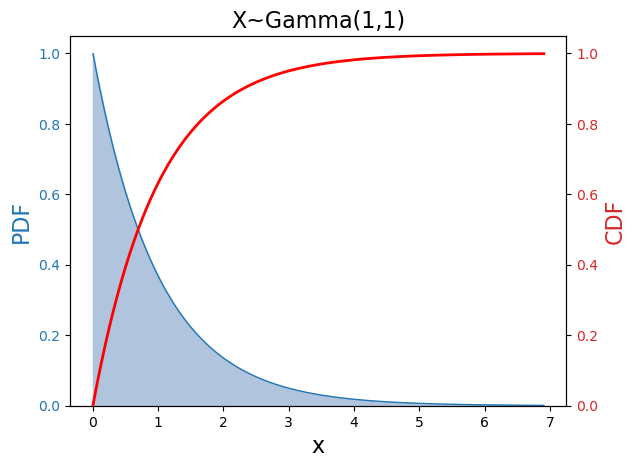
\includegraphics[scale=0.21]{Gamma-1-1.png}
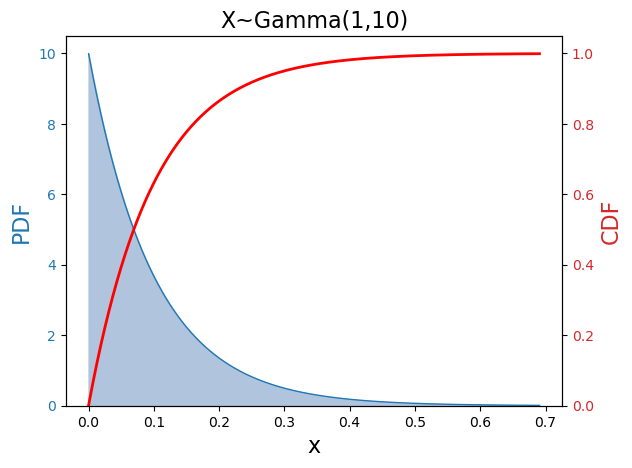
\includegraphics[scale=0.21]{Gamma-1-10.png}
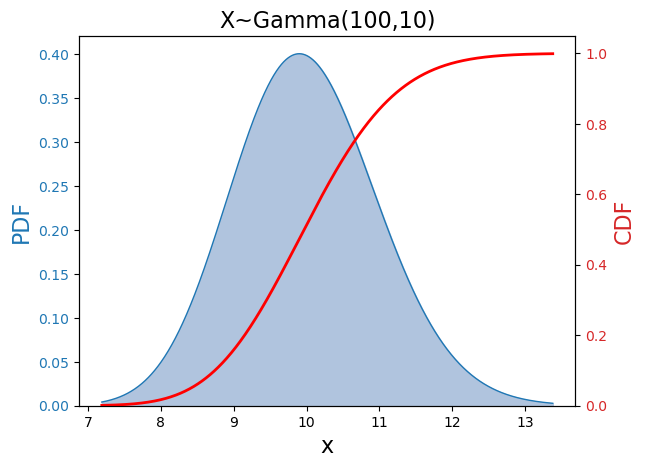
\includegraphics[scale=0.21]{Gamma-100-10.png}

The $\alpha$ is a shape hyper-parameter, and the $\beta$ is a scale.\\[1ex]

The \rbl{Expected Value} is $E[\theta]= \alpha \beta$ and the \rbl{Variance} is $V[\theta]= \alpha \beta^2$\\[1ex]
\end{frame}


\begin{frame}{Poisson-Gamma}
\small
Gamma priors:  \bbl{$\pi(\theta) \propto  \theta^{\alpha-1} e^{- \beta \theta}$}\\[1ex]
Poisson likelihoods: \gbl{$\mathcal{L}\wee{(y|\theta)}  \propto \theta^{n\,\overline{y}}  e^{-n\theta}$ }\\[1ex]
Gamma Posterior: \magtn{$Gamma(\alpha+n\overline{y}, \beta+n )$}\\[1ex]

%Posterior is Gamma($\alpha',\beta'$) with $\alpha' = \alpha+ n\overline{y}$ and $\beta' = \beta+ n$:\\[1ex]
%\magtn{$P(\lambda|y) \propto  \lambda^{\alpha+ n\overline{y} -1  } e^{-(\beta+n) \lambda}$}\\[1ex]

Note that for Gamma, the \rbl{Expected Value} is $E[\theta]= \alpha \beta$ and the \rbl{Variance} is $V[\theta]= \alpha \beta^2$\\[1ex]

Compare with Poisson $E[y]= \theta$ and $V[y]= \theta$\\[1ex]

For example, if we have Poisson data and guess at the rate parameter $\theta = 15$, we want $\alpha \beta = 15$ and $\alpha \beta^2 =  15$ ie $\alpha=15, \beta=1$.\\[1ex]
%We will use this for credible interval example.

\end{frame} 

\begin{frame}{Poisson-Gamma: \small$\magtn{Gamma(\bbl{\alpha}+}\gbl{n\overline{y}}\magtn{, \bbl{\beta}+}\gbl{n}\magtn{ )}  \propto \gbl{ \mathcal{L}(Data | \theta=15) } \times  \bbl{Gamma(\alpha, \beta)}   $}
\small
The static prior is \bbl{$Gamma(15,1)$}. True mean is \bbl{$\theta=15$}.\\[1ex]
%\only<1>{ \magtn{The Posterior is $Gamma(10+1\overline{y}, 1+1 )$ }  for \gbl{n=1 data point.}\\[1ex]} 
%\magtn{The Posterior updates with every new data point added. } \\

\begin{center}
\only<1> {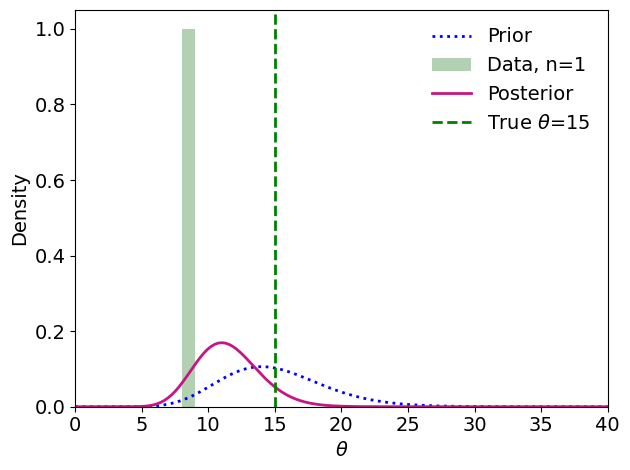
\includegraphics[scale=0.5]{hnPG-a15-b1-n1.png}}
\only<2> { 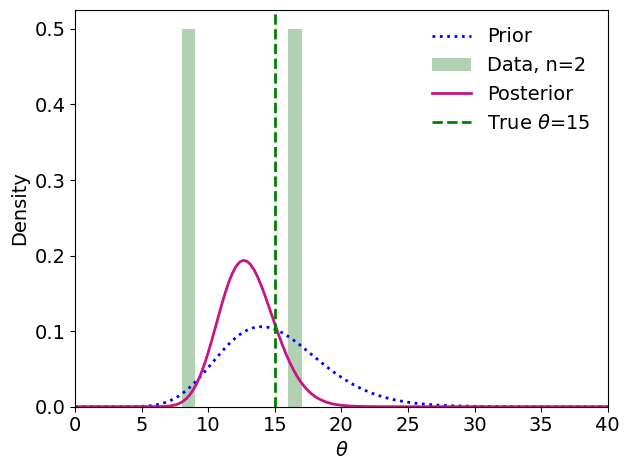
\includegraphics[scale=0.5]{hnPG-a15-b1-n2.png}}
\only<3> { 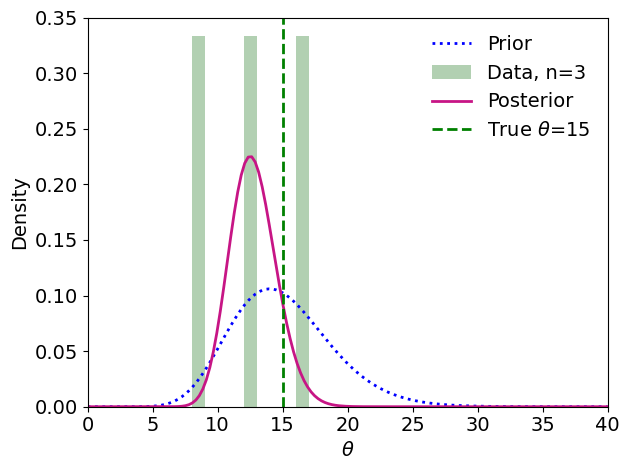
\includegraphics[scale=0.5]{hnPG-a15-b1-n3.png}}
\only<4> { 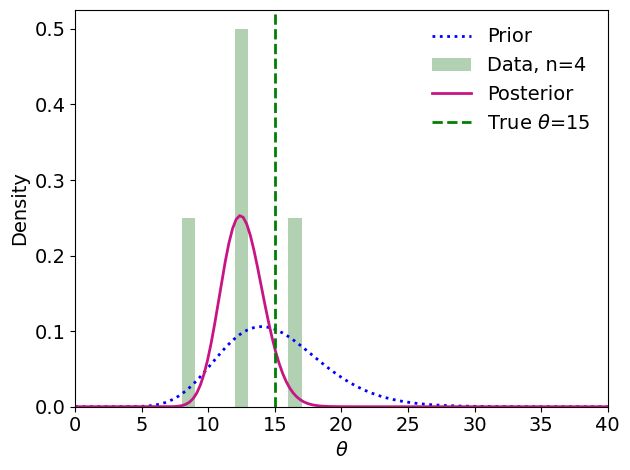
\includegraphics[scale=0.5]{hnPG-a15-b1-n4.png}}
\only<5> { 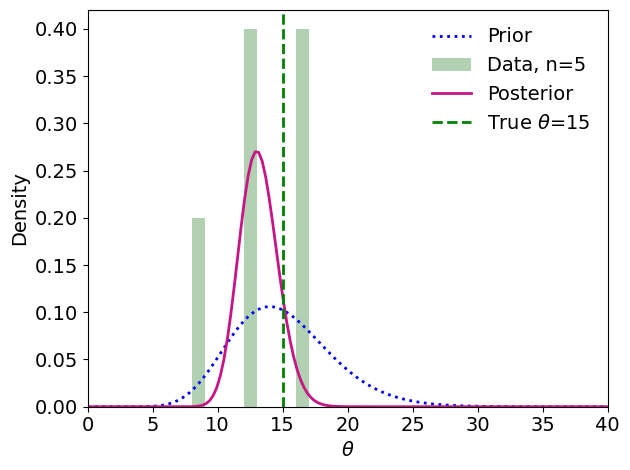
\includegraphics[scale=0.5]{hnPG-a15-b1-n5.png}}
\only<6> { 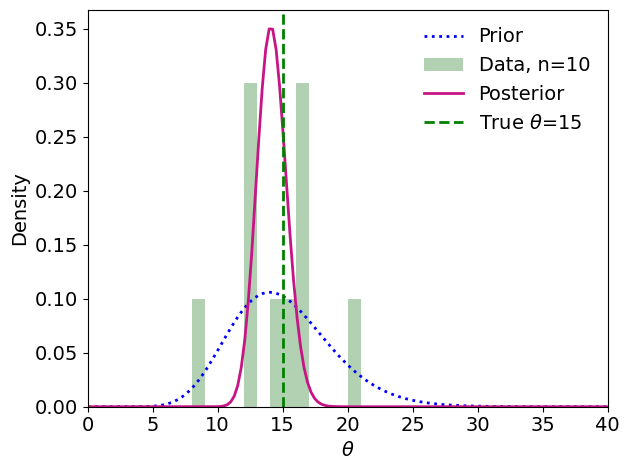
\includegraphics[scale=0.5]{hnPG-a15-b1-n10.png}}
\only<7> { 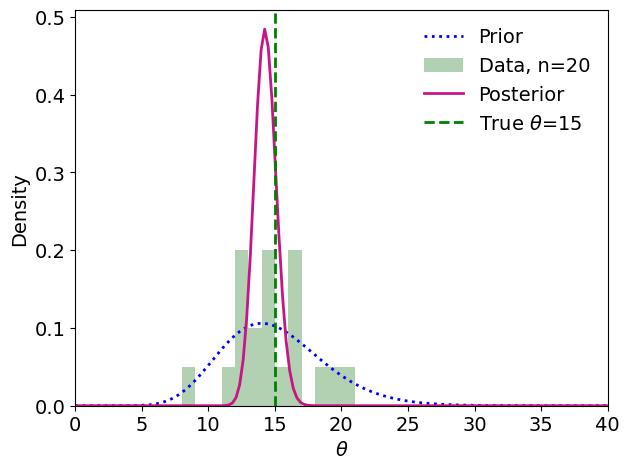
\includegraphics[scale=0.5]{hnPG-a15-b1-n20.png}}
\only<8> { 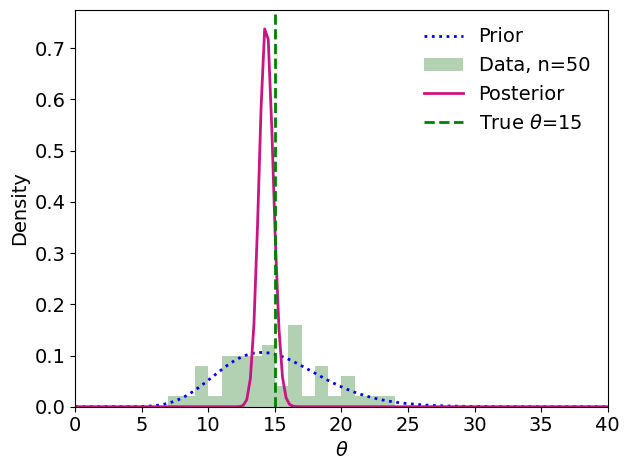
\includegraphics[scale=0.5]{hnPG-a15-b1-n50.png}}
\end{center}
\end{frame} 


\begin{frame}{Poisson-Gamma}
\small
What if we start with a really bad guess: \bbl{Gamma(1,1)}?:\\[1ex]

\begin{center}
\only<1> {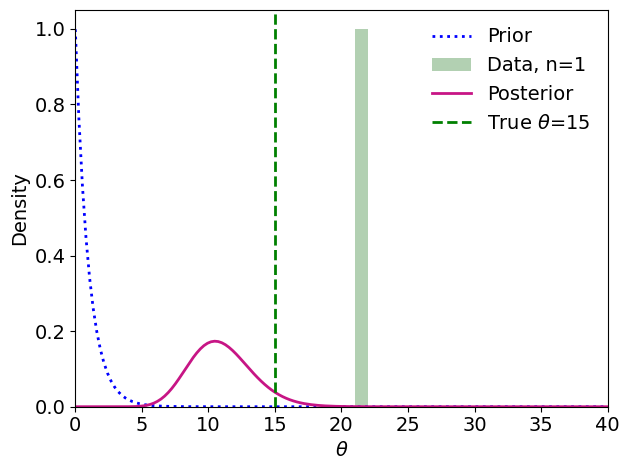
\includegraphics[scale=0.5]{hnPG-a1-b1-n1.png}}
\only<2> { 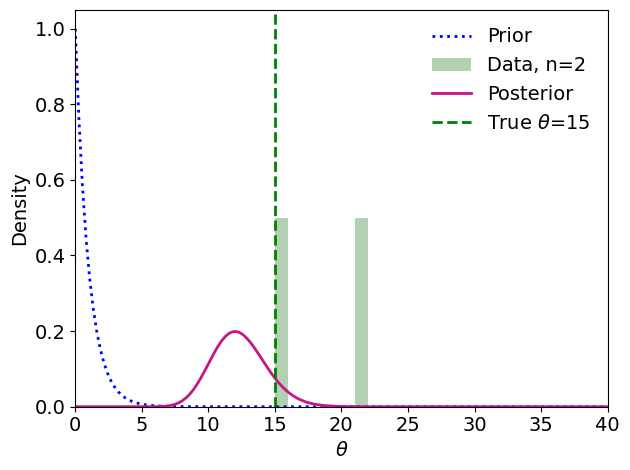
\includegraphics[scale=0.5]{hnPG-a1-b1-n2.png}}
\only<3> { 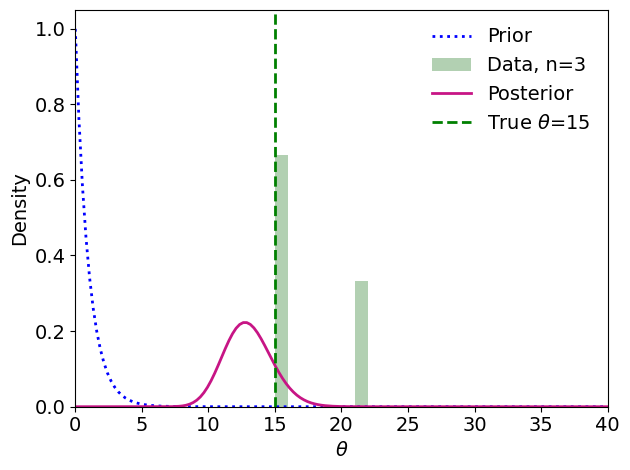
\includegraphics[scale=0.5]{hnPG-a1-b1-n3.png}}
\only<4> { 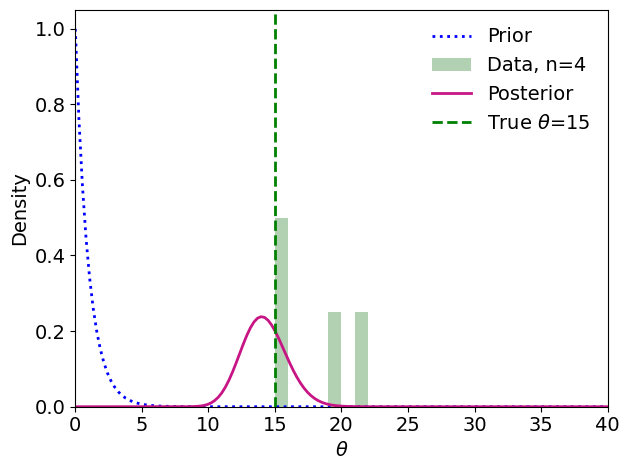
\includegraphics[scale=0.5]{hnPG-a1-b1-n4.png}}
\only<5> { 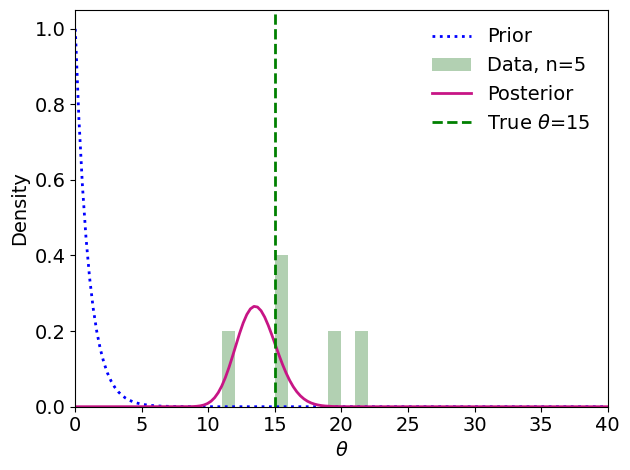
\includegraphics[scale=0.5]{hnPG-a1-b1-n5.png}}
\only<6> { 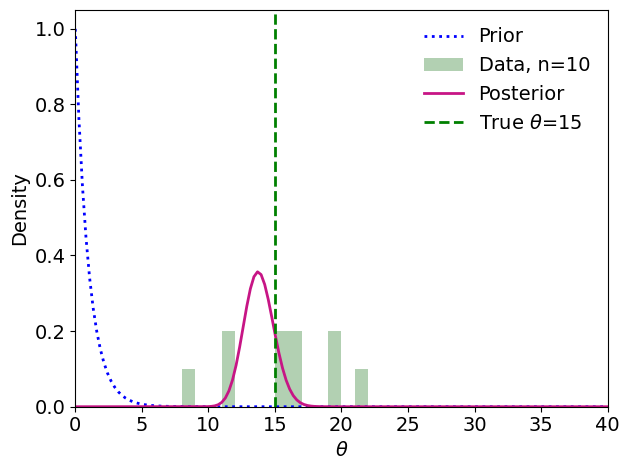
\includegraphics[scale=0.5]{hnPG-a1-b1-n10.png}}
\only<7> { 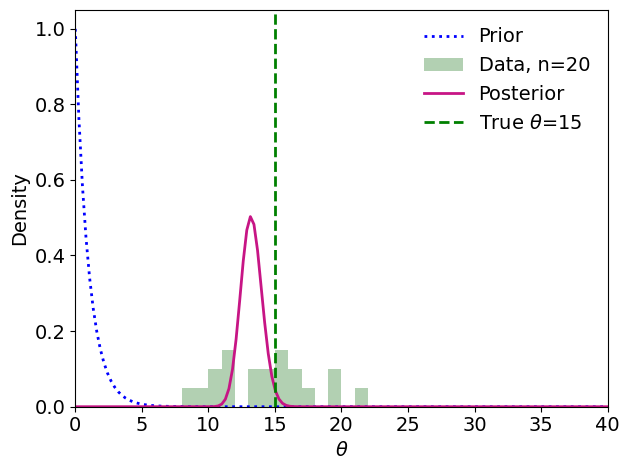
\includegraphics[scale=0.5]{hnPG-a1-b1-n20.png}}
\only<8> { 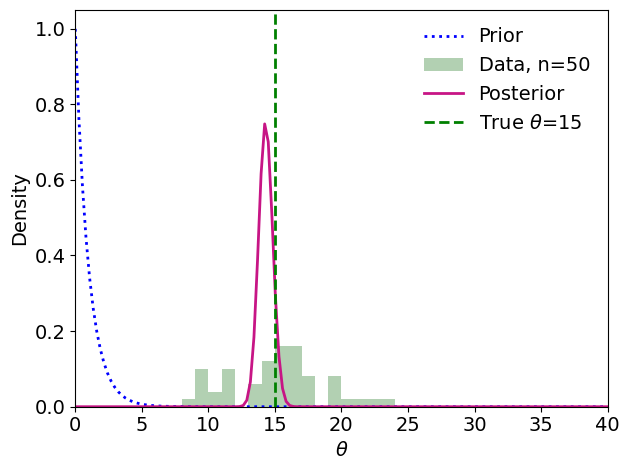
\includegraphics[scale=0.5]{hnPG-a1-b1-n50.png}}
\end{center}
\end{frame} 

\section*{Prediction}


\begin{frame}{Predictions}
\small
We have seen that we can use Bayes Updating to find a Posterior Probability that will give us a pretty good estimate of the mean of a distribution.\\[1ex]

The ingredients of the posterior are the Prior: what sort of distribution shape do we expect? and the Data itself.\\[1ex]

Helping the Data along with a Prior allows the Posterior to work well with even just a few events.\\[1ex]

If our prior is a bad guess, the posterior will take a little longer to converge, but quite quickly the information in the data overrides any mistakes in the prior.\\[1ex]

It would be so cool if we could predict the whole distribution, rather than just the mean. Which we can!

\end{frame} 


\begin{frame}{Predictions}
\small
\begin{itemize}
\item We have seen that we can use Bayes Updating to find a Posterior Probability that will give us a pretty good estimate of the mean of a distribution.
\item The ingredients of the posterior are the \bbl{Prior: what sort of distribution shape do we expect?} and the \gbl{Data} itself.
\item Helping the Data along with a Prior allows the Posterior to work well with even just a few events.
\item If our prior is a bad guess, the posterior will take a little longer to converge, but quite quickly \gbl{the information in the data overrides any mistakes in the prior}.
\item It would be so cool if we could predict the whole distribution, rather than just the mean. And we can!
\end{itemize}
\end{frame} 


\begin{frame}
\small
\begin{center}
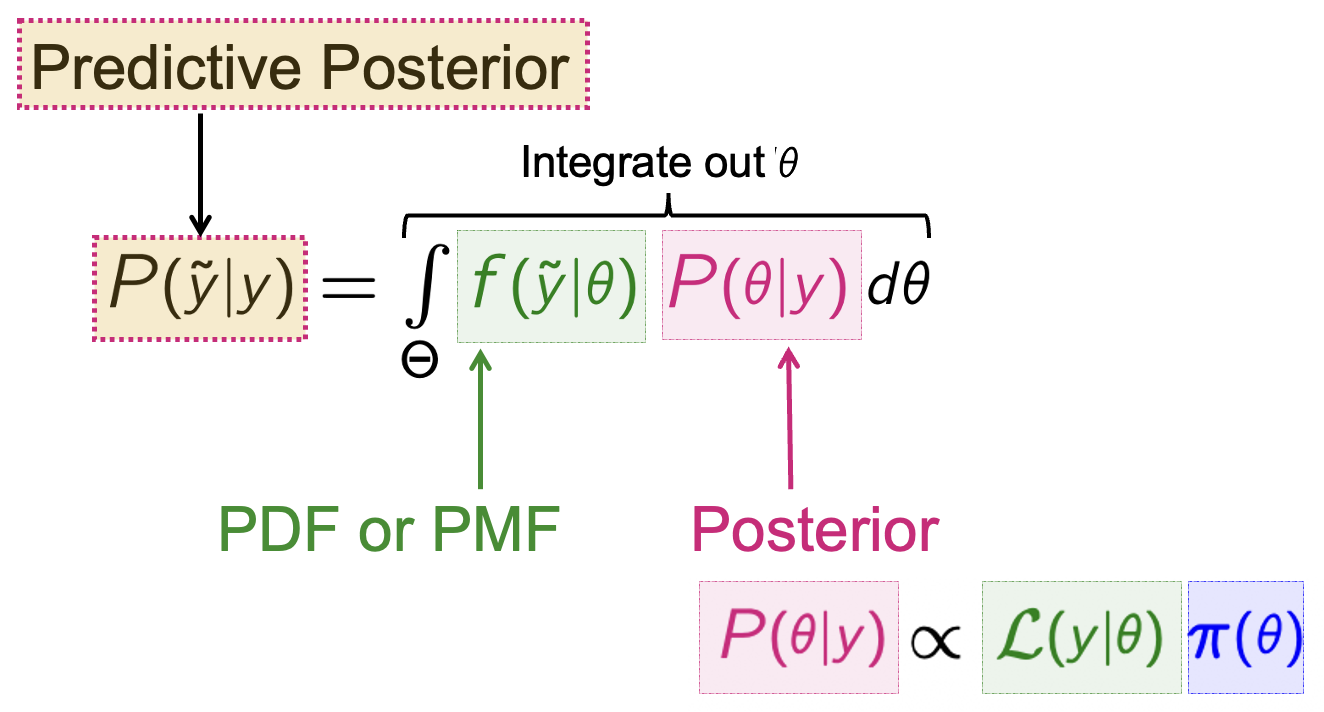
\includegraphics[scale=0.45]{predD.png}
\end{center}
\end{frame} 




\begin{frame}{Predictive Posterior}
\small
The (Marginal) \rbl{Predictive Posterior} describes the probability of a future measurement $\tilde{y}$, given our existing \gbl{pdf} and \magtn{posterior}, is:\\[1ex]

$P\wee{(\tilde{y} | y )} = \int\limits_{\Theta}  \gbl{ f\wee{(\tilde{y} | \theta )}}\; \magtn{P\wee{(\theta | y )} }\,  \wee{d\theta} $\\[1ex]

For Poisson-Gamma: $P(\tilde{y} | y ) = \int\limits_{0}^{\infty}  
\gbl{ e^{-\theta}\dfrac{\theta^{\tilde{y}}}{\tilde{y}!} }\; 
\magtn{ \dfrac{\beta'^{\alpha'}}{\Gamma(\alpha') } \theta^{\alpha'-1} e^{- \beta' \theta} }\,
\wee{d\theta}$,\\
where the hyper-parameters of the \magtn{Posterior Gamma} are $\alpha' = \alpha+n\overline{y}$ and $\beta' = \beta+n$\\[1ex]



%We find $P(\tilde{y} | y ) = \dfrac{1}{\tilde{y} !} \dfrac{\Gamma(\tilde{y}+\alpha) }{\Gamma(\alpha)}  ( 1- \mathcal{B} )^{\tilde{y}} \mathcal{B}^{\alpha}$, where $\mathcal{B} = \dfrac{\beta}{\beta+1}$\\[1ex]

The resulting Predictive $P(\tilde{y} | y )$ is a Negative Binomial:\\[1ex]
 $NBinom\left(\alpha+n\overline{y},  \dfrac{ \beta+n)}{(\beta+n+1)} \right)$\\

\end{frame} 




\begin{frame}{Predictive Posterior \hfill \small \grhl{ \texttt{ prediction = nbinom.pmf(xvals, n=n, p=p )}}}
\small
%The ( Marginal) Predictive Posterior for the true underlying distribution (sans prior) can be extracted by integrating the posterior. \\[1ex]
%
%A future measurement is $\tilde{y}$. 
%%Marginal PDF: $f_Y(y|\theta) = \int\limits_{s} f_{XY}(x,y|\theta) dx $\\[1ex]
%
%$P(\tilde{y} | y ) = \int\limits_{\Theta}  \gbl{ f(\tilde{y} | \theta )}  \magtn{ P(\theta | y)} d\theta $\\[1ex]
%
%The Posterior becomes peaked $P(\theta | y) \rightarrow \delta(\theta - \thetahat) $ (a Delta function, essentially a spike at the mean value). In this case we can write:\\[1ex]
%
%$P(\tilde{y} | y ) = \int\limits_{\Theta}  P(\tilde{y} | \theta )  \magtn{\delta(\theta - \thetahat) } d\theta  = P(\tilde{y} | \thetahat )$\\[1ex]

The Negative Binomial is just the Binomial, but for measuring failures rather than successes.
\begin{itemize}
\item Neg Binomial: $p_Y(y) \propto \theta^n (1-\theta)^y$  models the number of failures $y$. n is the number of successes, $\theta$ is the probability of one success. 
\item Binomial: $p_Y(y) \propto \theta^y (1-\theta)^{n-y}$  where $y$ is the number of successes and n is the total.
\end{itemize}
\vspace{0.2cm}

As a predictive prior for Poisson-Gamma, the parameters are:\\[1ex]
 \yhl{$n = \alpha+n\overline{y}$ and $p=\dfrac{ \beta+n)}{(\beta+n+1)}$}\\[1ex]

%\grhl{ \texttt{ from scipy.stats import nbinom}}

 
%The Negative Binomial distribution describes a sequence of i.i.d. Bernoulli trials, repeated until a predefined, non-random number of successes occurs, which in this case is our rate, $\lambda$.\\[1ex]
%n = a+(n*mean)
%p = (b+n)/(b+n+1)	
%prediction = nbinom.pmf(x, n=n, p=p )
\end{frame} 



\begin{frame}{Poisson-Gamma}
\small
Gamma priors:  \bbl{$\pi(\lambda) \propto  \theta^{\alpha-1} e^{- \beta \theta}$}\\[1ex]
Poisson likelihoods: \gbl{$\mathcal{L}\wee{(y|\theta)}  \propto \theta^{n\,\overline{y}}  e^{-n\theta}$ }\\[1ex]
Gamma Posterior: \magtn{$Gamma(\alpha+n\overline{y}, \beta+n )$}\\[1ex]
Neg Binom Predictive Posterior: \yhl{\magtn{$NBinom(\alpha+n\overline{y},  (\beta+n)/(\beta+n+1)  )$}}\\[1ex]

The Predictive Posterior is pretty neat, because unlike the Posterior which shrinks in variance around its mean value as the data increases, the predictive posterior remains the same shape as the data.
\end{frame} 






% PREDICTIVE POSTERIOR
\begin{frame}{Predictive Posterior}
\footnotesize

\begin{center}
\only<1> {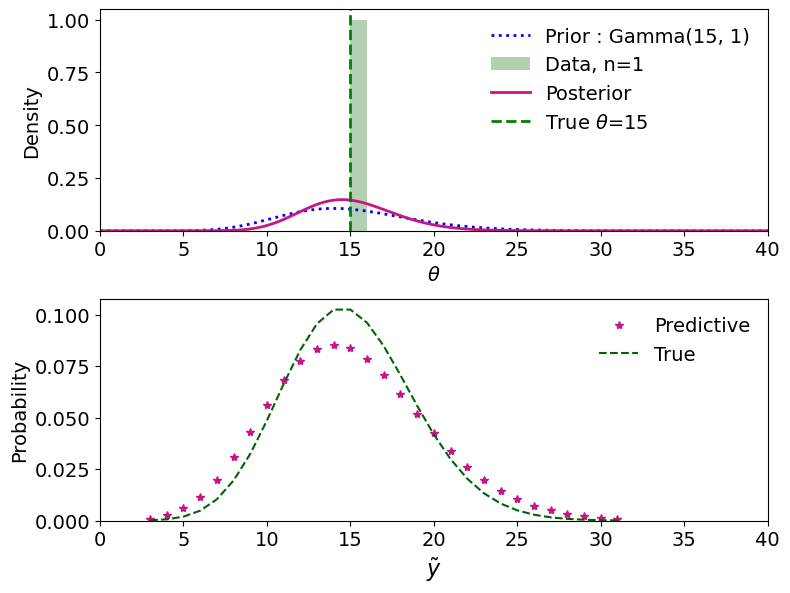
\includegraphics[scale=0.45]{predPG-a15-b1-n1.png}}
\only<2> { 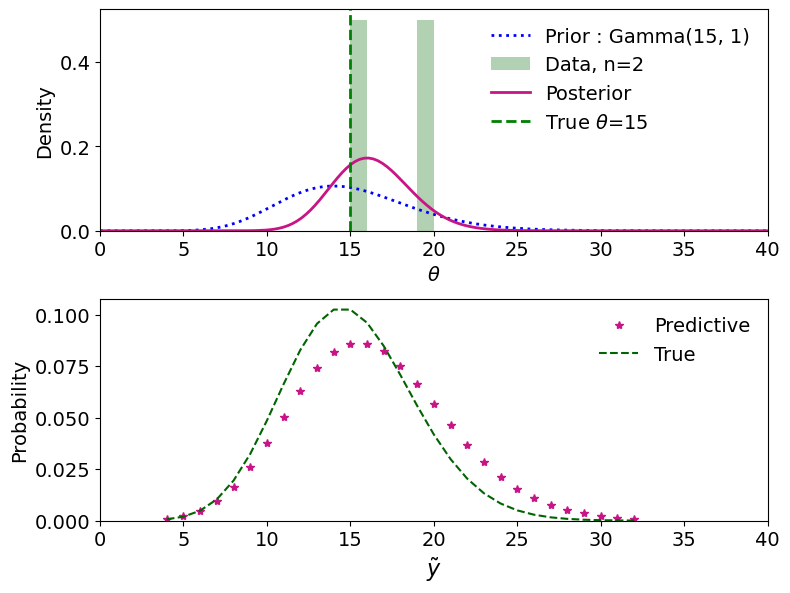
\includegraphics[scale=0.45]{predPG-a15-b1-n2.png}}
\only<3> { 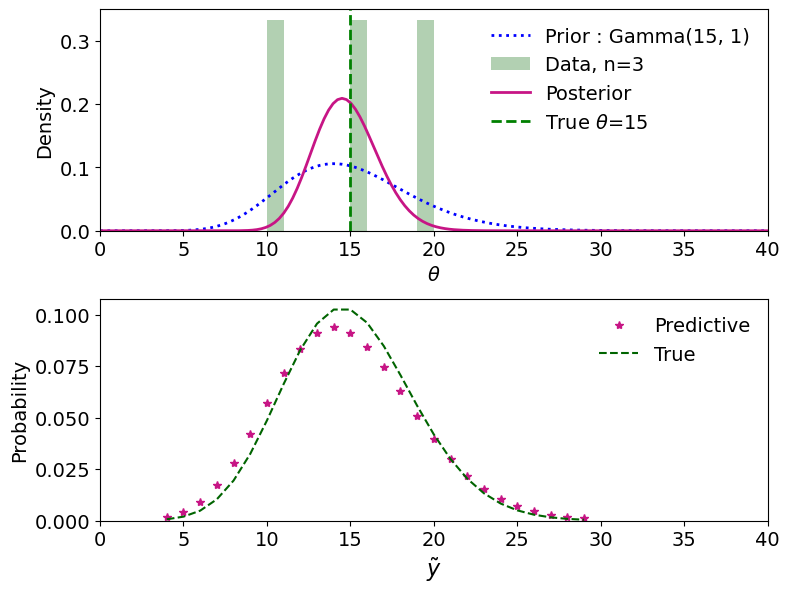
\includegraphics[scale=0.45]{predPG-a15-b1-n3.png}}
\only<4> { 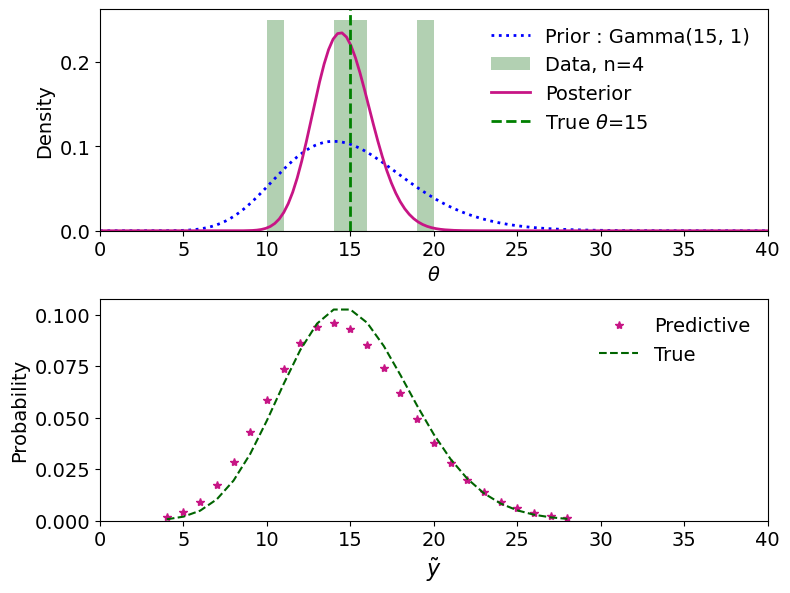
\includegraphics[scale=0.45]{predPG-a15-b1-n4.png}}
\only<5> { 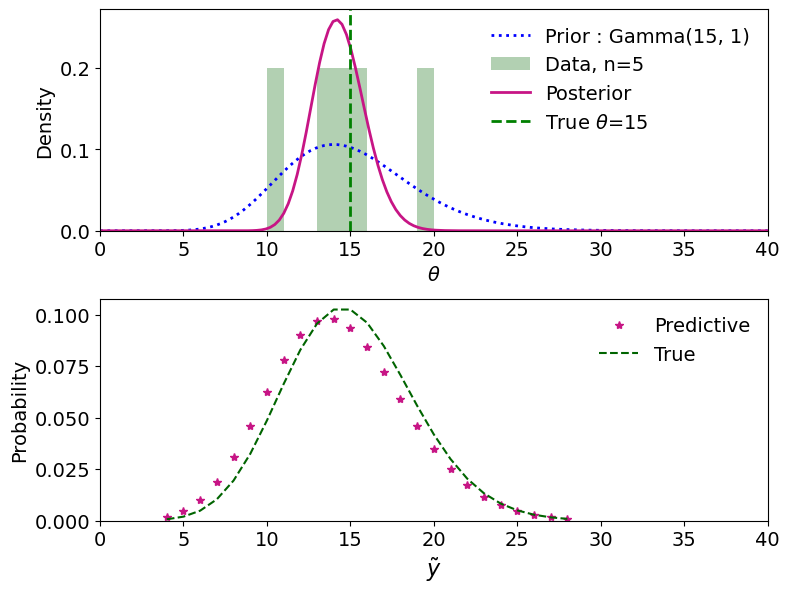
\includegraphics[scale=0.45]{predPG-a15-b1-n5.png}}
\only<6> { 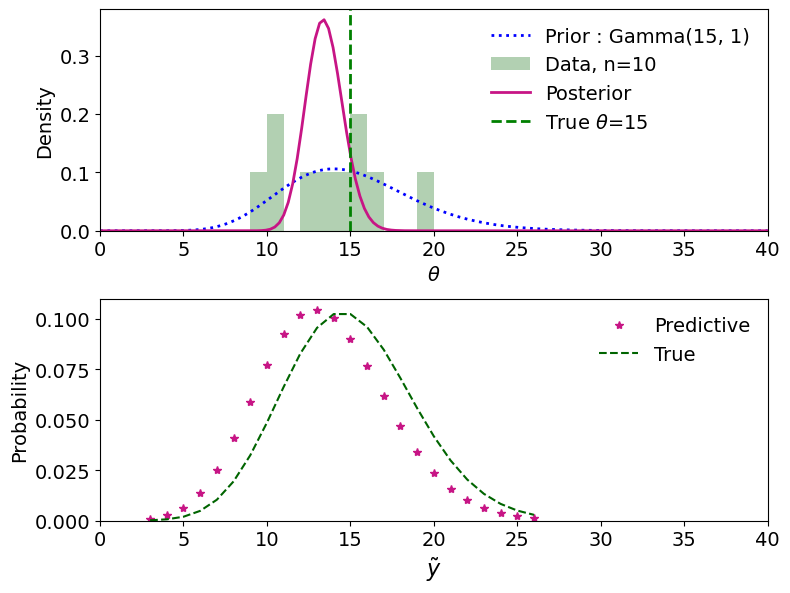
\includegraphics[scale=0.45]{predPG-a15-b1-n10.png}}
\only<7> { 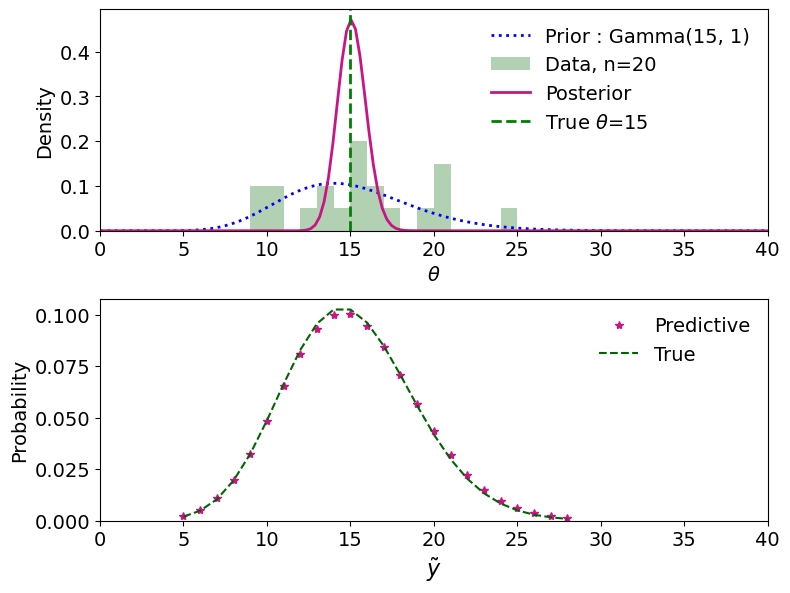
\includegraphics[scale=0.45]{predPG-a15-b1-n20.png}}
\only<8> { 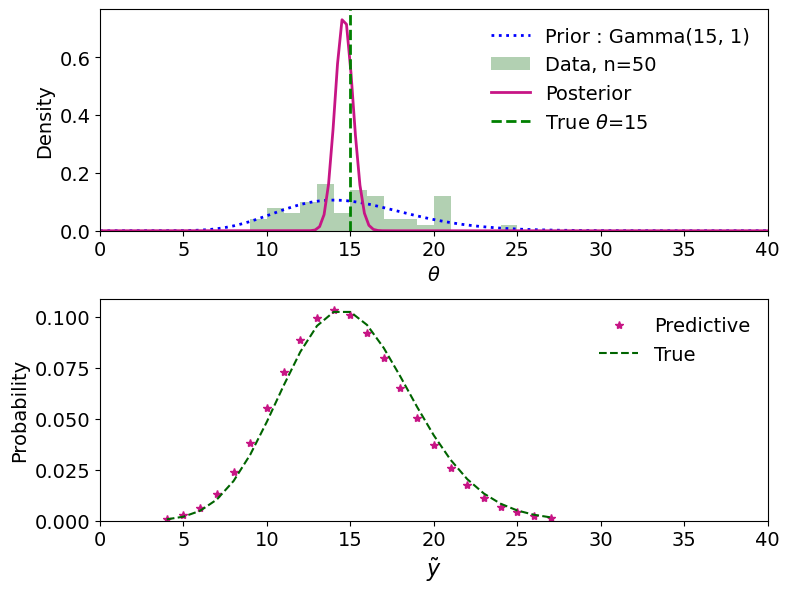
\includegraphics[scale=0.45]{predPG-a15-b1-n50.png}}
\end{center}
\end{frame} 


% PREDICTIVE POSTERIOR
\begin{frame}{Predictive Posterior with a daft prior}
\footnotesize

\begin{center}
\only<1> {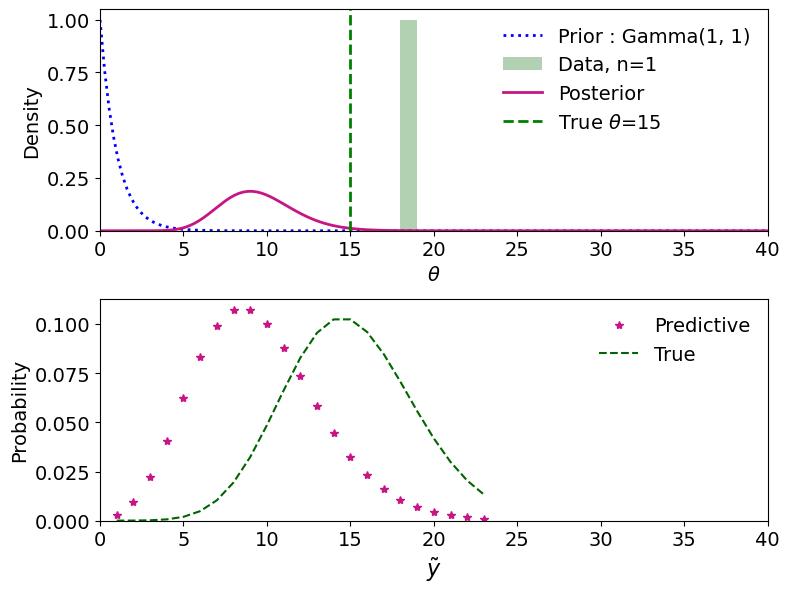
\includegraphics[scale=0.45]{predPG-a1-b1-n1.png}}
\only<2> { 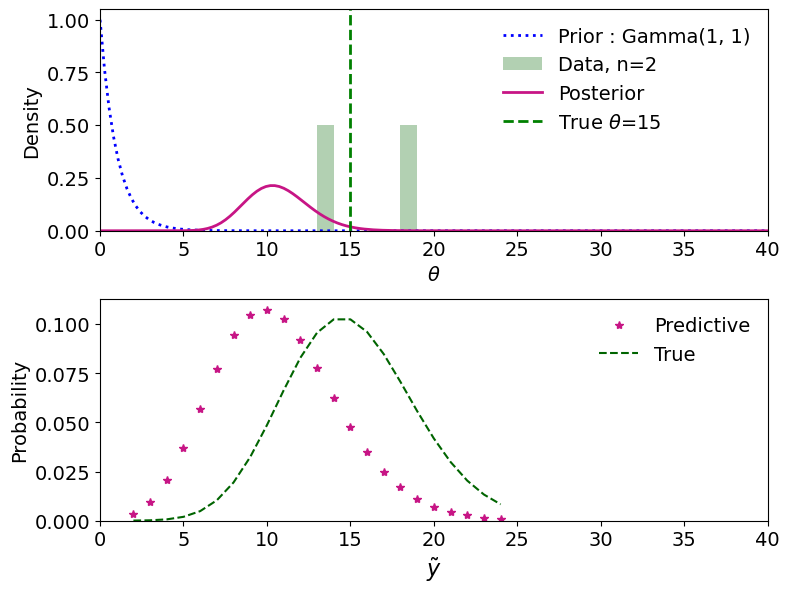
\includegraphics[scale=0.45]{predPG-a1-b1-n2.png}}
\only<3> { 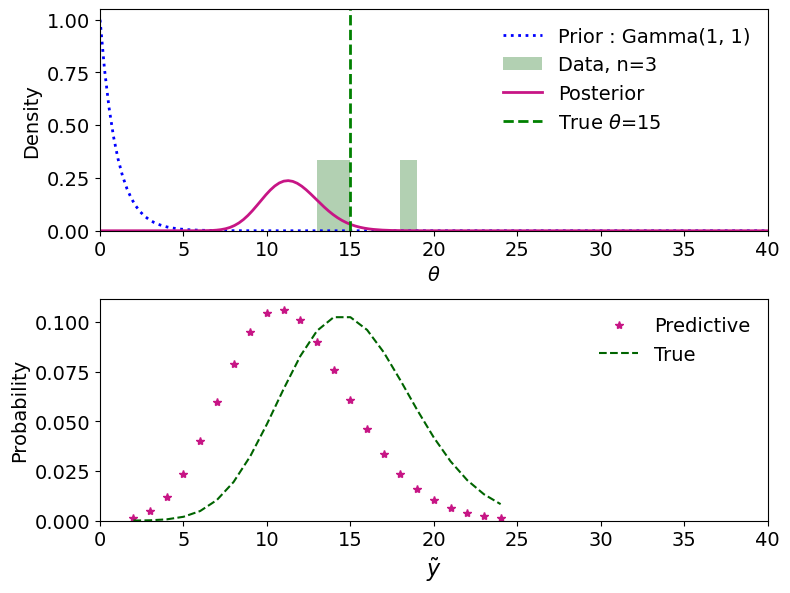
\includegraphics[scale=0.45]{predPG-a1-b1-n3.png}}
\only<4> { 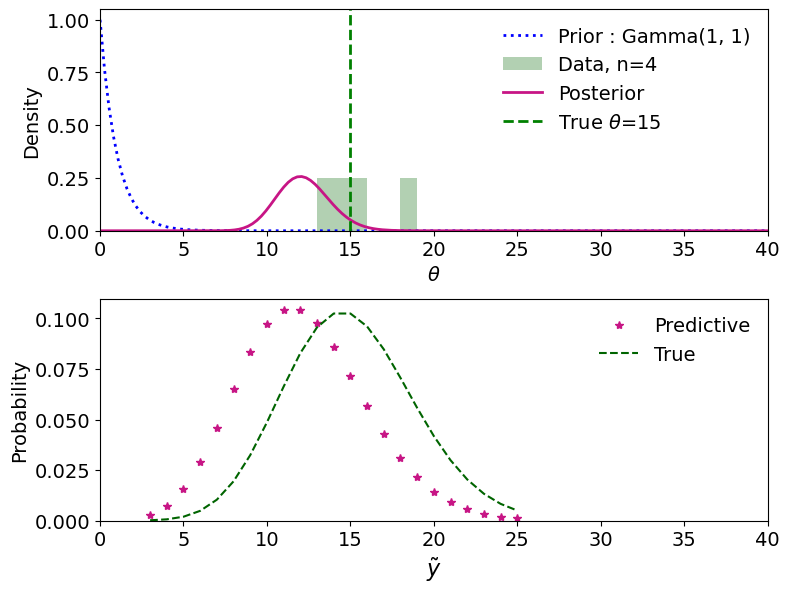
\includegraphics[scale=0.45]{predPG-a1-b1-n4.png}}
\only<5> { 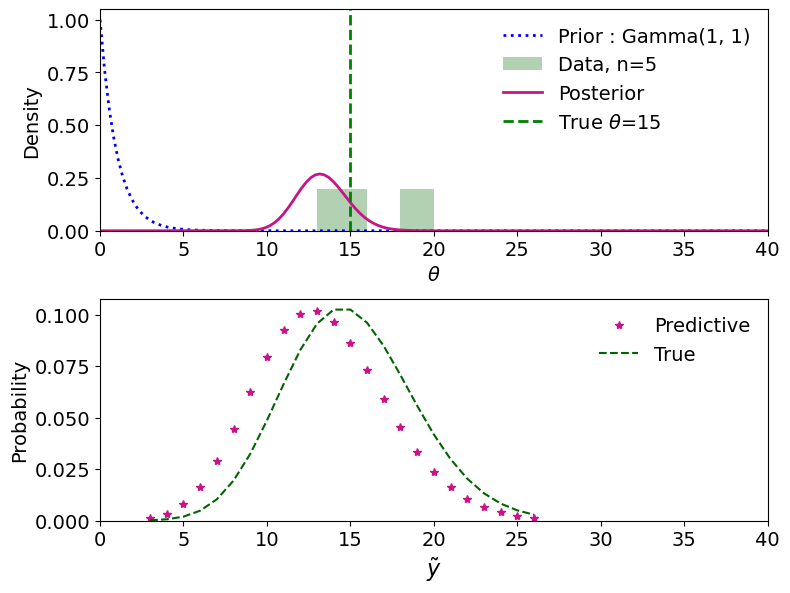
\includegraphics[scale=0.45]{predPG-a1-b1-n5.png}}
\only<6> { 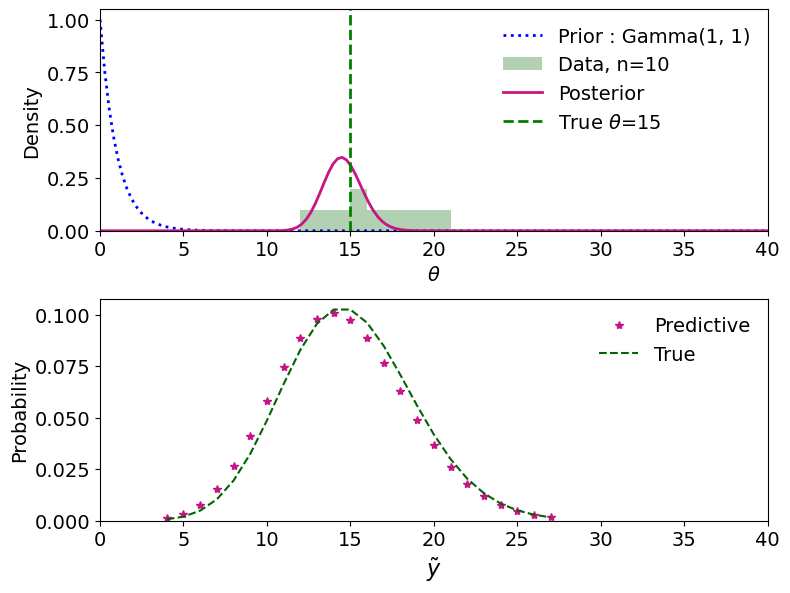
\includegraphics[scale=0.45]{predPG-a1-b1-n10.png}}
\only<7> { 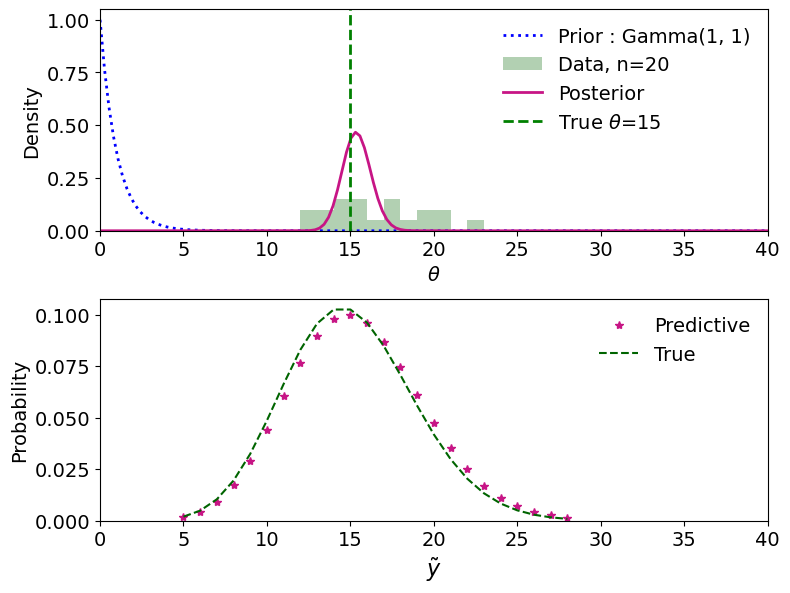
\includegraphics[scale=0.45]{predPG-a1-b1-n20.png}}
\only<8> { 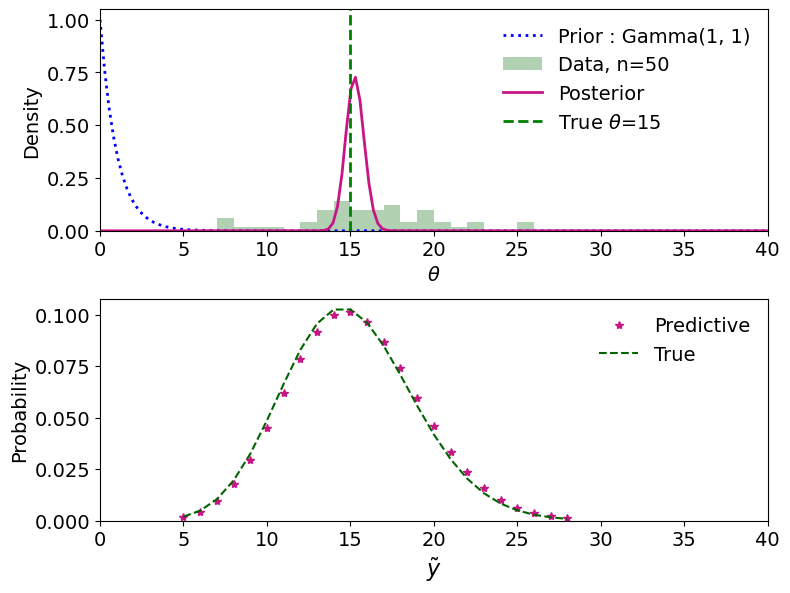
\includegraphics[scale=0.45]{predPG-a1-b1-n50.png}}
\end{center}
\end{frame} 



\begin{frame}{It's not Magic, it's Bayesian Updating.}
\small
The use of a Prior allows us to preserve the Uncertainty associated with measurements, particularly when N is small.\\[2ex]
The use of a Conjugate Prior makes the inference transparent and the analysis easy.\\[2ex]
If the Posterior integral is not a nice simple one, we can take samples from it using eg Markov Chain Monte Carlo, which will we look at next week.\\[2ex]
\end{frame}


%\begin{frame}{Multivariate Beta: Dirichlet }
%\small
%Multivariate Beta. \\ 
%Dirichlet(1,2,3):  Beta(1, 2+3) and Beta(2, 1+3) and Beta(3, 1+2)\\[1ex]
%Useful for categorical modelling eg is the favourite cake of my students coffee or carrot or red velvet.\\
%Categorical: what is the probability that student A's favourite cake is coffee cake?\\[1ex]
%
%Multinomial: what is the probability that DAT students' favourite cake is coffee cake?\\[1ex]
%
%Categorical $\rightarrow$ Multinomial as Bernoulli $\rightarrow$ Binomial.\\
%
%\end{frame} 










%\section*{MAP, Credible Intervals, Predictions}










%% MAP ESTIMATION
%\begin{frame}{Maximum A Posteriori Estimation}
%\small
%%The value of $\theta$ that maximises the Posterior distribution (the mode of the posterior) is the MAP estimate. \\[1ex]
%%
%%\begin{center}
%%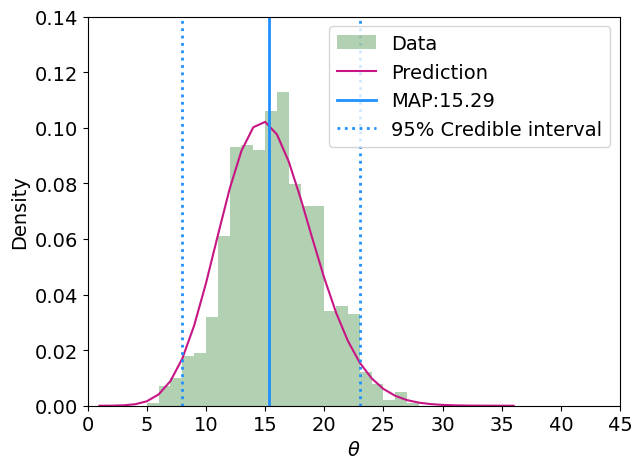
\includegraphics[scale=0.3]{mapPG-a15-b1.png}
%%\end{center}
%
%%Compare with MLE: MLE only uses the likelihood of the data, with no prior belief included.\\
%%
%%If MAP uses a uniform prior (an uninformative prior) then they are equivalent.\\
%
%The Decision Rule for MAP is to choose the hypothesis with the Highest Posterior Density.\\
%
%A HPD REGION is a Credible interval for which every value inside is higher than every value outside. This means it is the smallest possible Credible interval region.\\
%
%The Decision Rule for Minimum Cost is to choose the hypothesis with the lowest posterior risk.\\
%
%\end{frame} 





%% BAYES FACTOR
%\begin{frame}{Bayes Factor}
%\footnotesize
%The Bayes factor is the Likelihood ratio for two competing hypotheses.\\
%Posterior odds = prior odds times Bayes factor.\\
%If Bayes factor for H1/H0 is more than 1, then H1 is favoured by the data.\\
%\end{frame} 




\begin{frame}{Thanks For Your Time}
\center
\Huge
Fin.
\end{frame}

\end{document}